% artikkel_I_materialar.tex
% Artikkel I: Materialar som geopolitisk historie
% STOLAR-prosjektet - Kvantitativ designhistorie
% Spraak: Nynorsk
% v3 - mahogni-fokus, norske stolar, figurar

\documentclass[10pt, a4paper, twocolumn]{article}

\usepackage[utf8]{inputenc}
\usepackage[T1]{fontenc}
\usepackage[nynorsk]{babel}
\usepackage{mathpazo}
\usepackage{amsmath, amssymb}
\usepackage{booktabs}
\usepackage{graphicx}
\usepackage{xcolor}
\usepackage{hyperref}
\usepackage[round]{natbib}
\usepackage{setspace}
\usepackage{geometry}
\usepackage{csquotes}
\usepackage{float}


\geometry{margin=1.5cm, top=1.8cm, bottom=1.8cm, columnsep=0.6cm}
\setstretch{1.15}
\graphicspath{{fig/}}

\title{%
  \textbf{Mahogniens boge}\\[0.4em]
  \large Materialkurveanalyse og den koloniale dimensjonen i norsk stoldesign, 1280--2024%
}
\author{%
  Iver Raknes Finne\\
  \small Arkitektur- og designhøgskolen i Oslo (AHO)\\
  \small \texttt{iver.raknes.finne@stud.aho.no}
}
\date{}

\begin{document}
\maketitle

% ================================================================
\begin{abstract}
\noindent I perioden 1825--1849 inneheld \emph{kvar einaste registrerte stol} i Nasjonalmuseet si samling mahogni: 26 av 26 stolar, 100\,\%. Eit tropisk treslag frå Karibia og Mellom-Amerika har fullstendig utradert lokal materialvariasjon i den norske museale produksjonen. Denne artikkelen introduserer \textbf{materialkurveanalyse} for å kvantifisere dette fenomenet og sette det i eit 700-årig perspektiv. Ved hjelp av \textbf{Shannon-entropi} ($H'$) analyserer me materialbruken i 2\,284 stolar frå Nasjonalmuseet (NMK, $n = 671$) og Victoria and Albert Museum (V\&A, $n = 1\,613$). Entropien stig frå $H' = 1{,}0$ bits (1200-talet) til $H' = 5{,}07$ bits (1900-talet), men denne stiginga er ikkje monoton: mahogni-monopolet rundt 1800 representerer ein dramatisk entropikollaps i NMK-samlinga. Me namngjever dette \textbf{mahogniens boge} og demonstrerer at han er ein materialisert konsekvens av den transatlantiske kolonialhandelen. Funna syner at materialar er komprimerte geopolitiske historier: å lese ein stol sitt materialfelt er å lese eit verdskart.

\medskip
\noindent\textbf{Nøkkelord:} mahogniens boge, materialkurveanalyse, Shannon-entropi, kolonialisme, norsk stoldesign, Nasjonalmuseet, materialitet
\end{abstract}

\vspace{1em}
\hrule
\vspace{1.5em}


% ================================================================
\section{Ein stol, fem materialar, tre kontinent}

I magasinet til Nasjonalmuseet i Oslo står det ein stol registrert som OK-10330A, datert til om lag 1830. Materiallista er kort: \emph{fernissert mahognifiner, intarsia i kvitved, hestehårstrekk}, med ein berande konstruksjon av eik og furu. For ein konvensjonell designhistorikar er dette ein anonym historismestol. Men materiallista er ikkje anonym. Ho er eit komprimert verdskart.

\emph{Mahognien} kjem frå tropiske regnskogar i Karibia eller Mellom-Amerika, felt av tvangsarbeidande menneske under det britiske kolonistyret og frakta over Atlanterhavet i eit handelsnettverk som omsette sukker, slavar og tømmer i same rørsle. \emph{Hestetaglet} knyter stolen til europeiske leverandørkjeder for animalske fiber. \emph{Furu} og \emph{eik} veks i skogane kring snekkarverkstaden. Éin stol. Fem materialar. Tre kontinent.

\begin{figure}[H]
  \centering
  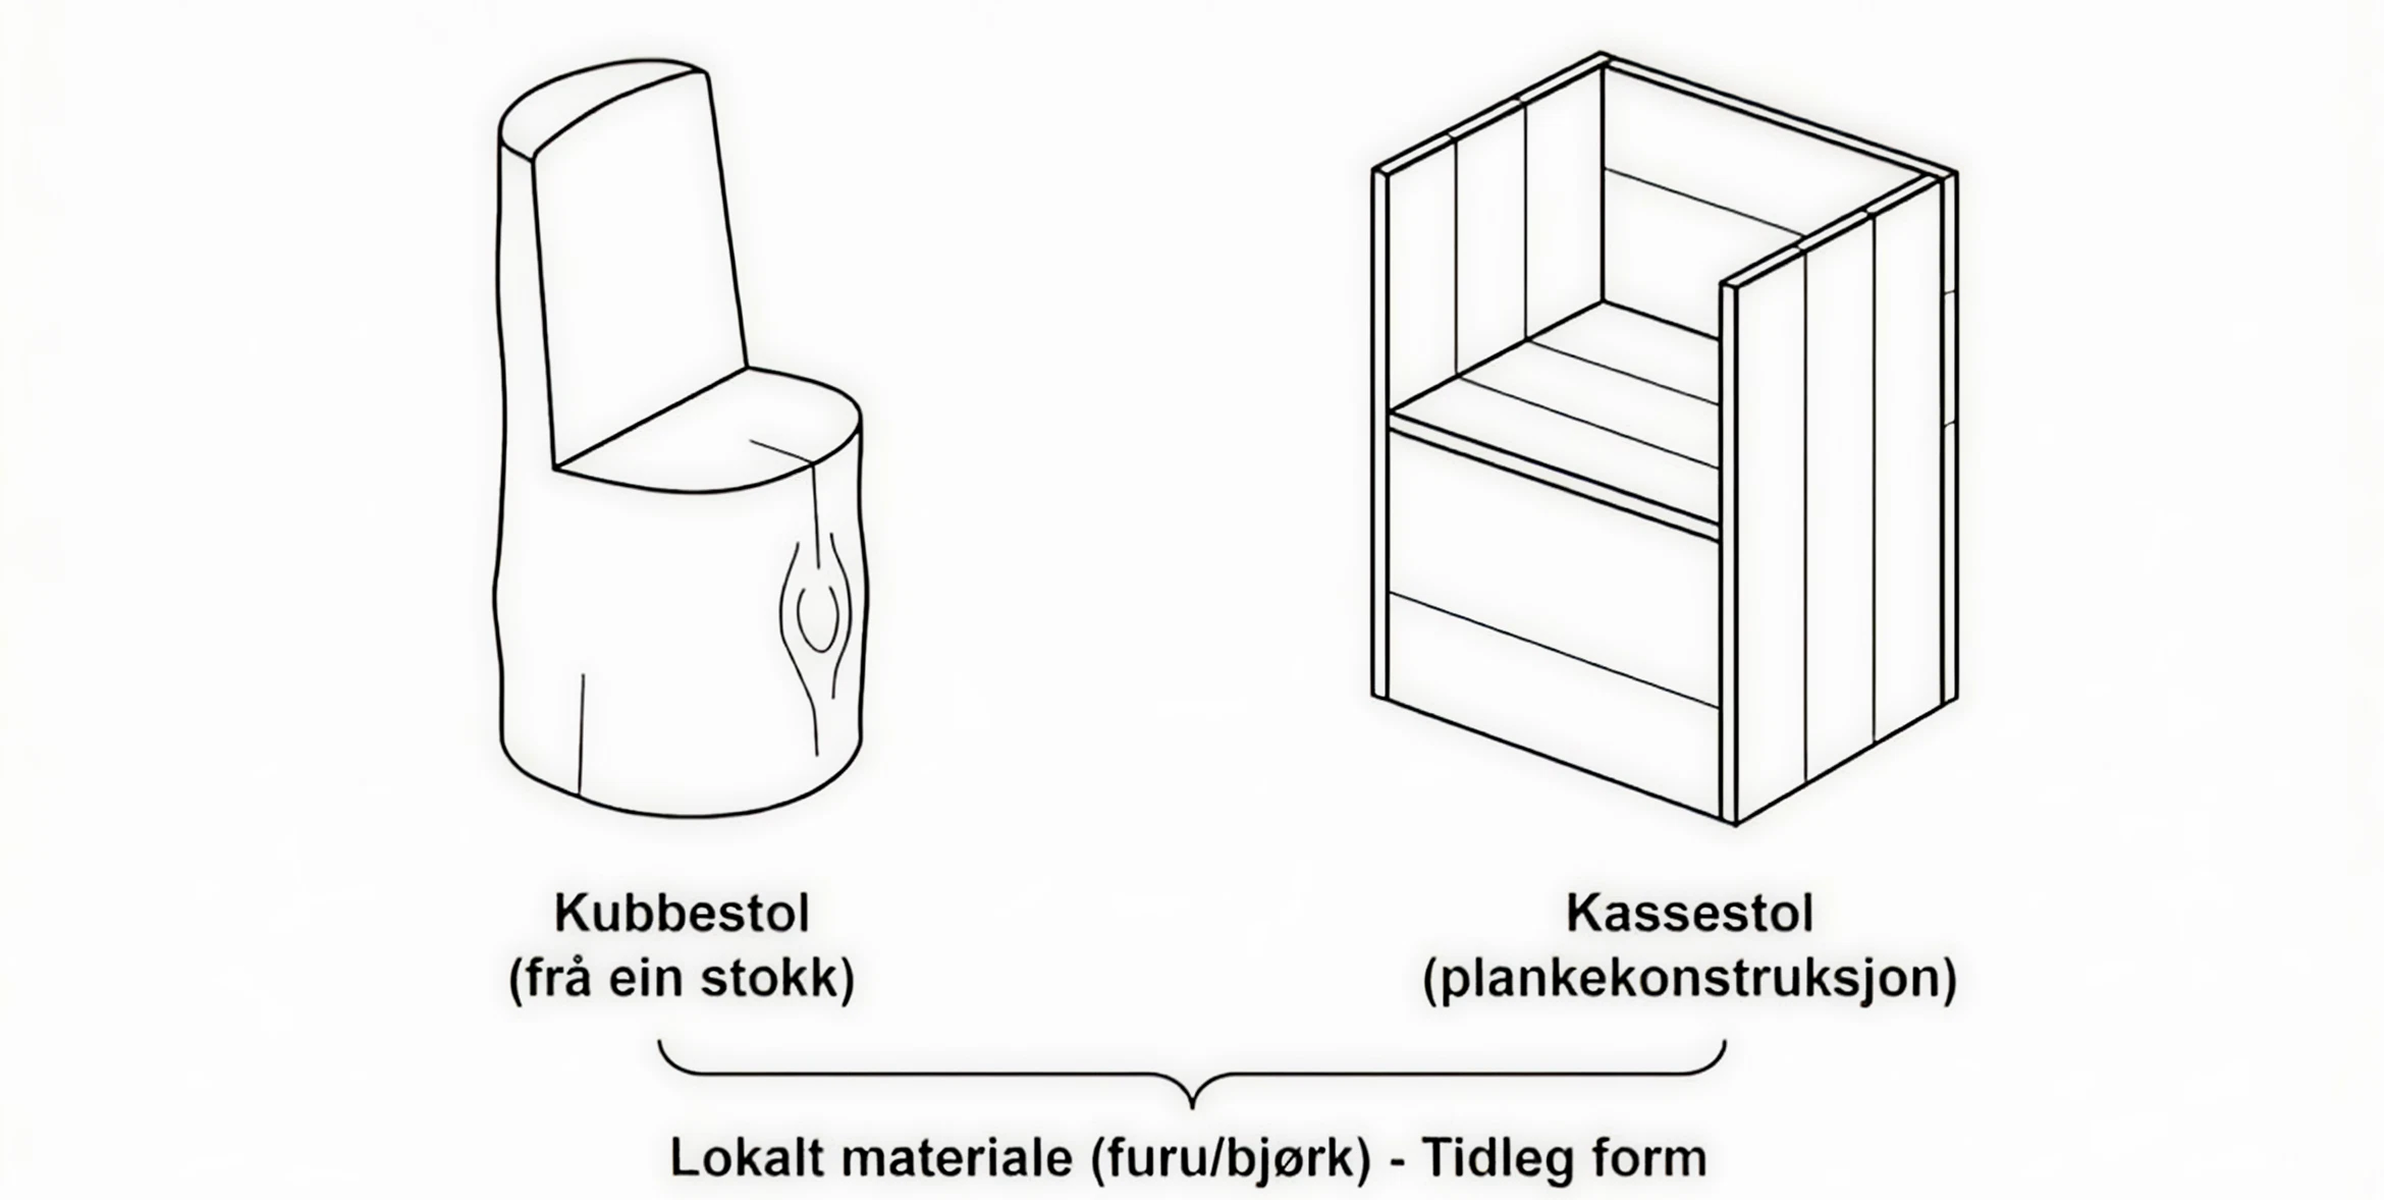
\includegraphics[width=\columnwidth]{teikn_kubbestol.png}
  \caption{Kubbestol (fraa ein stokk) og kassestol (plankekonstruksjon). Begge brukar lokalt materiale (furu/bjork). Gaarastolen er ein kassestol.}
  \label{fig:kubbestol}
\end{figure}

550 år tidlegare, i Bø i Telemark, vart \textbf{Gårastolen} (OK-10700) skapt av to materialar: \emph{bjørk} og \emph{furu}. Det er ein kassestol i stolpekonstruksjon med utskoren dekor og ferniss, truleg frå perioden 1280--1350. Begge tresortar veks i dei same dalføra der stolen vart laga. Materialradien var nokre få kilometer. Mellom Gårastolen og empirestolen ligg ikkje berre 550 år, men ei omvelting i korleis verda er organisert: frå lokalt kretslaup til globalt nettverk.

Denne artikkelen måler denne omveltinga kvantitativt, med mahogniens boge i den norske Nasjonalmuseet-samlinga som det sentrale empiriske funnet.

\begin{figure}[H]
  \centering
  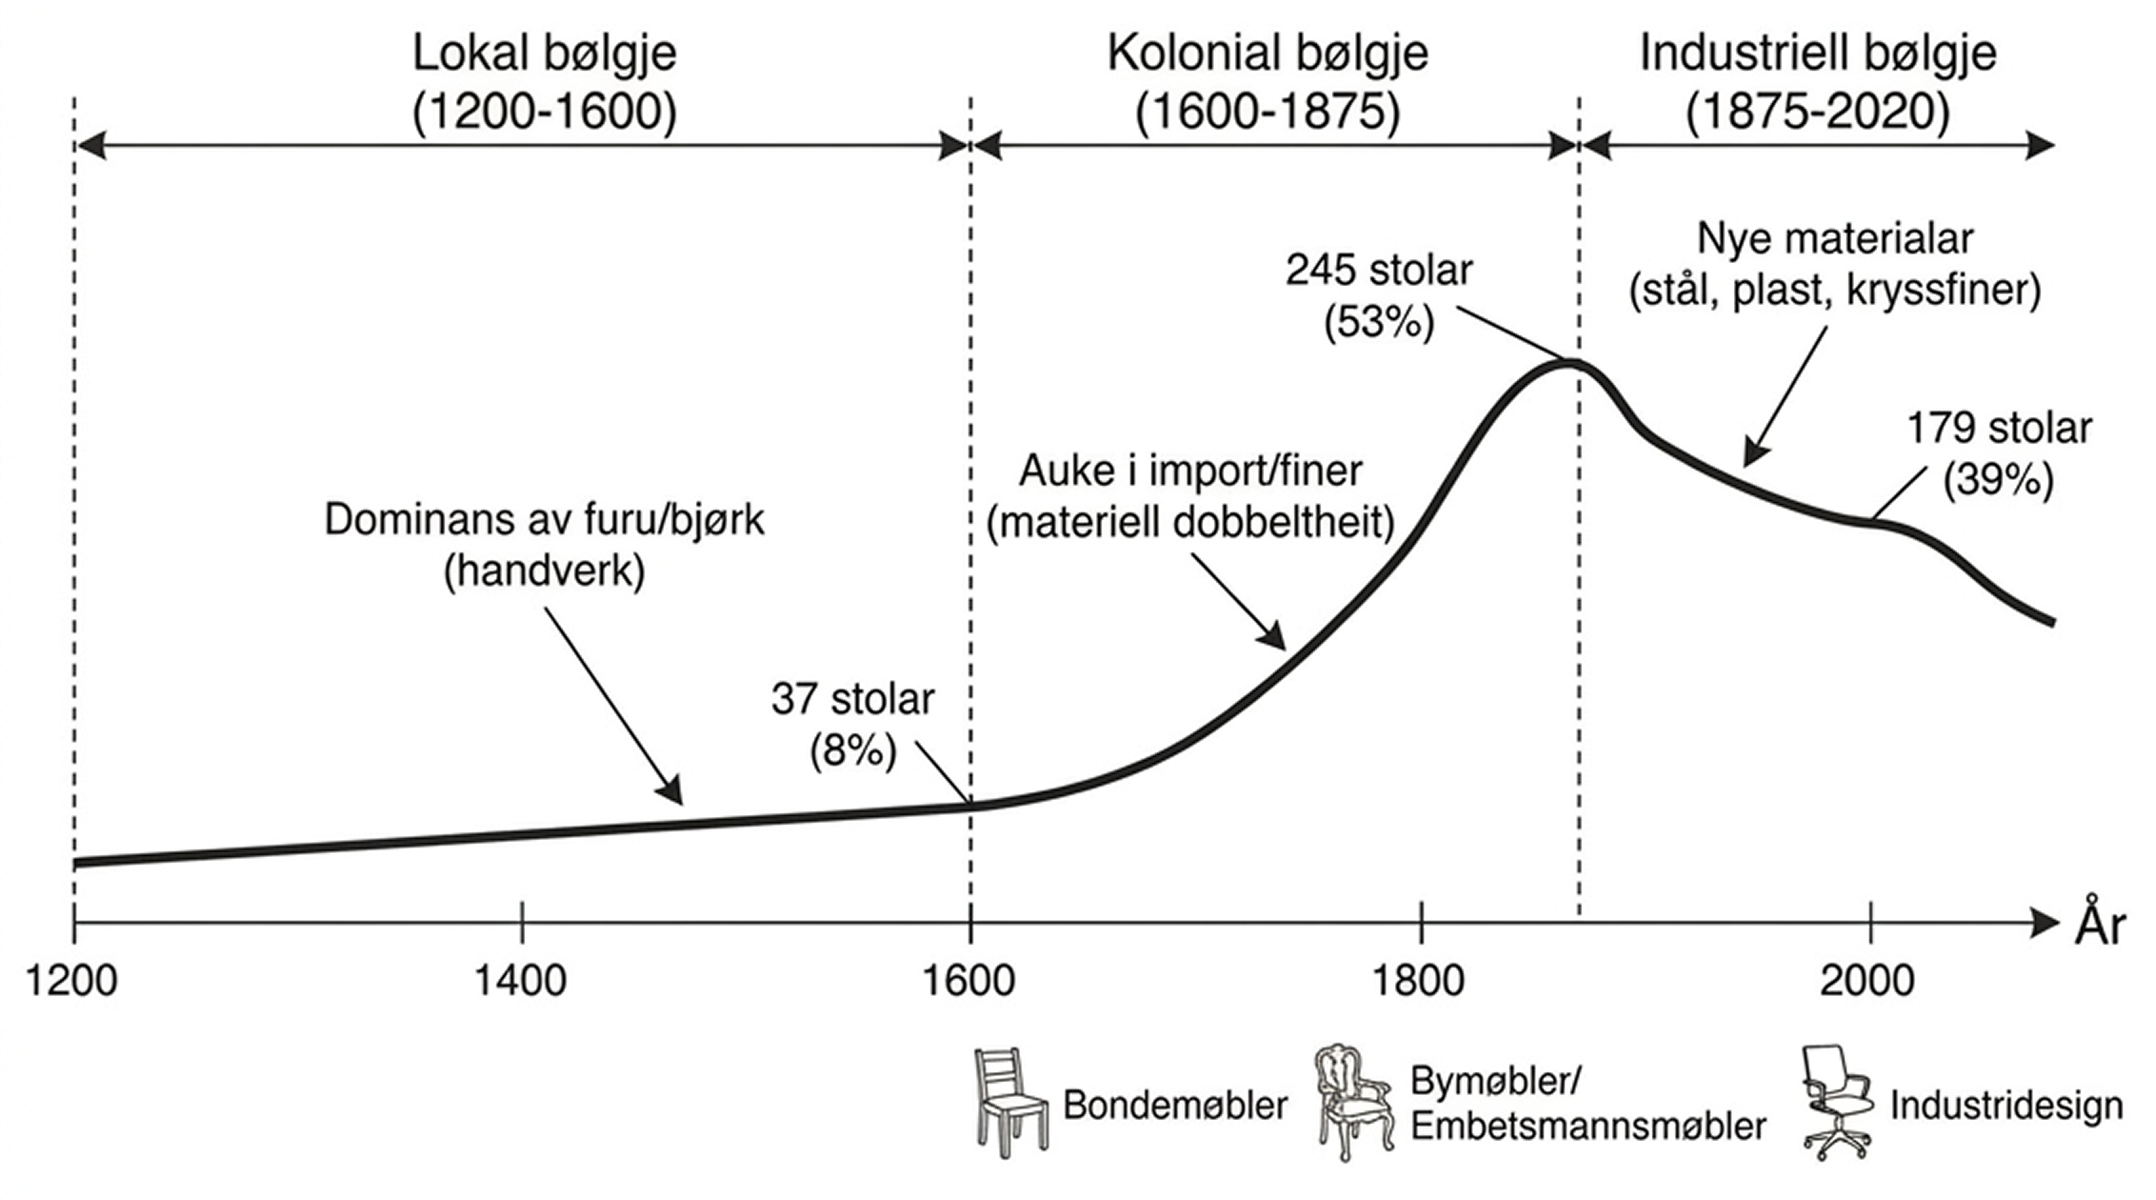
\includegraphics[width=\columnwidth]{teikn_kolonial_bolgje.png}
  \caption{Tre materialbolgjer: lokal (1200--1600), kolonial (1600--1875) og industriell (1875--2020). Toppunktet ved 245 stolar (53\,\%) markerer det koloniale klimakset. Bondemoblar, bymoblar og industridesign representerer ulike sosiale lag.}
  \label{fig:bolgje}
\end{figure}


% ================================================================
\section{Teori: materialar som geopolitiske spor}

\subsection{Den materielle sivilisasjonen}

\citet{braudel1979} viste i sitt trebandsverk \emph{Civilisation mat\'erielle} korleis kvardagslege ting avspeglar dei djupaste strukturane i verdssystemet. Møblar, klede og matvarer er ikkje perifere uttrykk for djupare strukturar; dei \emph{er} strukturane, materialiserte i gjenstandar. Ein stol er ikkje ein refleksjon av ein økonomi; han er eit fragment av den. Braudel kalla dette \textbf{den materielle sivilisasjonen}: det laget av menneskeleg aktivitet der produksjon, forbruk og kvardagspraksis kryssar kvarandre i konkrete objekt.

\subsection{Verdsystemteori og materialstraumar}

\citet{wallerstein2004} presiserte den geopolitiske mekanismen: i eit verdsystem flyt råvarer frå \emph{periferi} til \emph{sentrum}, medan ferdigvarer flyt i motsett retning. Denne asymmetrien er ikkje tilfeldig, men strukturelt betinga av maktrelasjonar. Tropisk tømmer (mahogni, ibenholt, palisander) reiser frå karibiske og søramerikanske skogar til europeiske verkstader; ferdige møblar reiser frå London til Kristiania. Materialstraumen ber med seg ein implisitt maktgeografi som vert innskriven i sjølve gjenstanden.

Som \citet{mintz1985} demonstrerte for sukker, er ein tilsynelatande uskyldig vare ofte spegelen til eit brutalt maktsystem. Sukker og mahogni reiste i same skip, produserte av same tvangsarbeidskraft, finansierte av same handelskapital. Å analysere mahogni sin posisjon i norske museumssamlingar er difor ikkje berre eit materialhistorisk prosjekt, men eit \emph{postkolonialt}. \citet{anderson1995} har argumentert spesifikt for at mahogni var ein ``luxury commodity'' der etterspørselen i Europa aktivt dreiv avskoginga og tvangsarbeidet i Karibia.

\subsection{Tre materialkategoriar}

\citet{manzini1986} skilde mellom materialar som vert \emph{funne} i naturen og materialar som vert \emph{konstruerte} i laboratoriet. Me legg til ein tredje kategori, inspirert av Wallerstein: materialar som vert \emph{importerte} gjennom imperiale nettverk. Desse tre kategoriane definerer tre materialepokar som korresponderer med tre geopolitiske regime:

\begin{enumerate}
  \item \textbf{Funne materialar} (1200--1600): bjørk, furu, eik, nøttetre. Henta frå det lokale landskapet. Materialradien er avgrensa til gangavstand.
  \item \textbf{Importerte materialar} (1600--1900): mahogni, ibenholt, palisander, rotting, silke. Transporterte gjennom koloniale forsyningskjeder. Materialradien er interkontinental.
  \item \textbf{Konstruerte materialar} (1900--): stål, kryssfiner, plast, glasfiber, polypropylen. Syntetiserte i industrielle prosessar. Materialradien er global, men abstrahert frå geografi.
\end{enumerate}

\subsection{Affordanse og formkanalisering}

\citet{gibson1977} definerte \textbf{affordanse} som dei handlingsmoglegheitene eit miljø tilbyr ein organisme. Kvart materiale har sine affordansar: bjørk kan bøyast men ikkje sveisast; stål kan sveisast men ikkje skjerast med handverktøy; plast kan sprøytestøypast til nær alle geometriar. Når eit nytt materiale kjem inn i verkstaden, endrar det ikkje berre \emph{kva} stolen er laga av, men \emph{kva former} som er moglege. Mahogni sin hardheit og finkornetheit mogeleggjorde relieffskjering og finering som norske treslag ikkje tola; ibenholt si tettheit mogeleggjorde tynne innleggsdetaljar.

\citet{ashby2013} formaliserte dette gjennom \textbf{materialvalgkart}: fleiraksa diagram der eigenskapar som stivheit, vekt og kostnad definerer kva materialar som er tilgjengelege for ein gitt funksjon. Kvar epoke har sine tilgjengelege regionar i dette kartet, og desse regionane utvidar seg irreversibelt over tid. Entropi-kurva me presenterer i resultatdelen er, i denne forstand, eit einaksig samandrag av det fleiraksa materialvalgkartet sin ekspansjon.

\subsection{Informasjonsteori som materielt verktøy}

Shannon-entropi \citep{shannon1948} vart opphavleg utvikla for å kvantifisere informasjon i kommunikasjonskanalar, men har sidan vorte eit standardverktøy i biologisk økologi for å måle artsmangfald \citep{magurran2004}. Overføringa til designhistorie er ikkje vilkårleg: eit materialøkosystem og eit biologisk økosystem er begge komplekse system der mangfald er ein emergent eigenskap av underliggjande seleksjonstrykk. Der økologen spør ``kor mange artar finst, og kor jamt er dei fordelte?'', spør me ``kor mange materialar finst, og kor jamt er dei fordelte?'' Svaret gjev oss eit kvantitativt mål på den materielle kompleksiteten i ein gitt epoke.


% ================================================================
\section{Metode}

\subsection{Datagrunnlag}

\textbf{STOLAR-databasen} \citep{finne2026} inneheld 2\,284 stolar med gyldige material- og tidsdata frå to europeiske museumssamlingar:

\begin{itemize}
  \item \textbf{Nasjonalmuseet} (NMK, Oslo): $n = 671$ stolar. Hovudsakleg norsk møbelhistorie.
  \item \textbf{Victoria and Albert Museum} (V\&A, London): $n = 1\,613$ stolar. Internasjonal dekorativ kunst med britisk tyngdepunkt.
\end{itemize}

For mahogni-analysen splittar me NMK-dataa i 25-årsbolkar for å fange dynamikken med høgare oppløysing enn hundreårsbolkar.

\subsection{Materialkurveanalyse}

Me introduserer \textbf{materialkurveanalyse} som ein kvantitativ metode med tre komponentar: Shannon-entropi ($H'$), Pielou-jamnheit ($J'$) og Jaccard-avstand ($d_J$).

\textbf{Shannon-entropi} \citep{shannon1948} i bits:
\begin{equation}
  H' = -\sum_{i=1}^{S} p_i \log_2 p_i
\end{equation}

\begin{quote}
\textbf{Shannon-entropi i kontekst:} Tenk deg at du plukkar opp ein tilfeldig stol frå 1280 og prøver å gjette materialet. Du treng eitt ja-eller-nei-spørsmål: bjørk eller furu? Det er éin bit. Plukk opp ein stol frå 1900-talet, og du treng over fem spørsmål. Uvissa har vorte femdobla. \emph{Shannon-entropi måler kor overraskande det typiske materialvalet er.}
\end{quote}


% ================================================================
\section{Resultat}

\subsection{Mahogniens boge}

Figur~\ref{fig:mahogni} syner det mest slåande funnet i denne studien.

\begin{figure}[H]
  \centering
  
\includegraphics[width=\columnwidth]{fig1_mahogni_boge.pdf}
  \caption{Mahogniens boge: andel stolar med mahogni i NMK-samlinga, 25-årsbolkar. Kulminasjonspunktet ved 100\,\% i 1825--1849 markerer det historiske toppunktet for kolonial materialimport til Noreg.}
  \label{fig:mahogni}
\end{figure}

I perioden 1825--1849 inneheld \textbf{100\,\% av alle registrerte NMK-stolar mahogni}: 26 av 26 stolar. Eit tropisk treslag har oppnådd fullstendig materialmonopol i den norske museale stolproduksjonen. Bogen har ein karakteristisk asymmetri: han stig gradvis frå 8,3\,\% i 1600--1624, akselererer til 61,7\,\% i 1800--1824, kulminerer ved 100\,\% i 1825--1849, og fell deretter tilbake gjennom 37,8\,\% (1850--1874) til 5,3\,\% (1875--1899) og null etter 1975.

Denne bogen er ikkje ein stilistisk preferanse. Det er eit \textbf{materielt avtrykk av den transatlantiske handelsøkonomien}. The Naval Stores Act av 1721 fjerna tollsatsar paa tropisk hardved og demokratiserte tilgangen utover London. Kulminasjonen i 1825--1849 fell saman med perioden etter abolisjonen av slaveriet i det britiske imperiet (1833/34). Kollapsen reflekterer den globale uttomminga av kommersiell mahogni, som forte til at alle tre \emph{Swietenia}-artane vart plasserte paa CITES sine vernelister. Toppunktet fell saman med perioden der Storbritannia sin kontroll over karibisk og sentralamerikansk tømmer var på sitt sterkaste, og der norske snikkarar hadde størst tilgang til mahogni gjennom britiske mellomledd. Fallet etter 1850 korresponderer med utarming av dei lett tilgjengelege tropiske skogane og framveksten av industrielle erstatningsmateriaal.

Me kan identifisere fem fasar i bogen:

\begin{enumerate}
  \item \textbf{Introduksjon (1600--1699):} Mahogni dukkar opp sporadisk (8,3\,\% i 1600--1624, deretter null i fleire periodar). Materialet er ein kuriositet, ikkje ein standard.
  \item \textbf{Akselerasjon (1700--1799):} Mahogni etablerer seg. I 1700--1724 har 25,6\,\% av NMK-stolane mahogni. Andelen oscillerer mellom 10\,\% og 25\,\%, dreven av svingingar i handelsvolum og norske importørar si tilknyting til britiske tømmermarknader.
  \item \textbf{Kolonial kulminasjon (1800--1849):} Eksponentiell vekst: 61,7\,\% i 1800--1824, 100\,\% i 1825--1849. Mahogni har oppnådd fullstendig materialhegemoni. Kvar einaste stol som vert vurdert verdig å ta vare på i Nasjonalmuseet frå denne perioden, er ein mahognistol.
  \item \textbf{Tilbaketrekking (1850--1899):} Raskt fall: 37,8\,\% i 1850--1874, 5,3\,\% i 1875--1899. Avskoging, endra handelsruter, og framveksten av nasjonalromantiske materialideal driv mahogni ut.
  \item \textbf{Utslokking (1900--):} Mahogni held seg sporadisk til 1950, deretter null. Industrielle materialar har gjort kolonialtreet overflødig.
\end{enumerate}

\subsection{Mahogni per tiår: finare oppløysing}

Når me bryt ned til tiårsbolkar (tabell~\ref{tab:decade}), vert dynamikken endå tydelegare. Mahogni-andelen i heile databasen (ikkje berre NMK) følgjer ein logistisk vekstkurve:

\begin{table}[H]
\centering
\caption{Mahogni-andel per tiår, alle stolar i databasen. Toppunktet i 1760-åra (69\,\%) representerer det absolutte høgdepunktet for mahogniens boge i den britiske samlinga.}
\label{tab:decade}
\begin{tabular}{@{}lrrr@{}}
\toprule
\textbf{Tiår} & \textbf{N stolar} & \textbf{Med mahogni} & \textbf{Andel} \\
\midrule
1700--1709 & 111 & 27 & 24,3\,\% \\
1720--1729 &  67 &  7 & 10,4\,\% \\
1740--1749 &  31 & 12 & 38,7\,\% \\
1750--1759 & 118 & 68 & 57,6\,\% \\
1760--1769 &  42 & 29 & \textbf{69,0\,\%} \\
1780--1789 & 100 & 48 & 48,0\,\% \\
1800--1809 & 102 & 40 & 39,2\,\% \\
1820--1829 &  36 & 21 & 58,3\,\% \\
1840--1849 &  27 & 15 & 55,6\,\% \\
1870--1879 &  63 &  8 & 12,7\,\% \\
1900--1909 &  89 & 13 & 14,6\,\% \\
1930--1939 &  98 &  5 &  5,1\,\% \\
\bottomrule
\end{tabular}
\end{table}

Toppunktet i \emph{heile databasen} (inkludert V\&A) fell i 1760-åra (69\,\%), som korresponderer med det britiske imperiet sin territoriale ekspansjon i Karibia etter sjuårskrigen (1756--1763). I NMK-samlinga kjem toppunktet seinare (100\,\% i 1825--1849), noko som stadfestar at Noreg er ein sekundærmottakar: den koloniale materialstraumen når periferien med ei forseinking på 60--80 år.

\subsection{Cubamahogni: artsnivået}

Materialkommentar-feltet i databasen gjev oss endå finare oppløysing. 19 stolar har spesifisert \emph{cubamahogni} (\emph{Swietenia mahagoni}), alle frå OK-10888-serien (ca.\ 1820). Ytterlegare 24 stolar er beskriven med \emph{mahognifiner} (tynn fasade finert på billegare tre), 21 med \emph{mahogni finert på bøk}, 11 med \emph{beiset mahogni} (lokalt tre farga for å imitere mahogni), og berre 2 med \emph{massiv mahogni}. Denne graderinga avslører eit firedelt hierarki av kolonialt materialengasjement:

\begin{enumerate}
  \item \textbf{Massiv cubamahogni} (2 stolar): Heile stolen er hogd frå importert tre. Dyrast, mest prestisjefull, og mest materialintensiv.
  \item \textbf{Cubamahogni finert på bøk/eik} (19 stolar): Berande konstruksjon i lokalt tre, men overflata er ekte cubamahogni. OK-10888-serien si materialresept.
  \item \textbf{Mahognifiner} (24 stolar): Tynn fasade, uklart om det er cubamahogni eller andre mahogni-artar. Eit kompromiss mellom prestisje og pris.
  \item \textbf{Beiset mahogni} (11 stolar): Lokalt tre (ofte bøk) \emph{farga for å sjå ut som mahogni}. Den billegaste kolonialsimulakringen. Materiell dobbeltheit vert her materiell \emph{løgn}: treet gjev seg ut for å vere noko det ikkje er.
\end{enumerate}

Materiell dobbeltheit er altså ikkje eit binært fenomen; det er eit kontinuum frå autentisk til imitert, frå kolonialt monopol til kolonialt teater.

\subsection{Mahogni-hestetagl-koplinga}

Blant dei 474 mahognistolane i databasen har 87 (18,4\,\%) hestetagl som polstringsfyll. Denne koplinga er ikkje tilfeldig: mahogni er eit hardt, finkornet treslag som gjev ein glatt, kald overflate. Stolen \emph{krev} polstring for komfort. Hestetagl var det mest tilgjengelege polstringsfyllet i europeiske leverandørkjeder. Materialkommentarane stadfester dette: ``fernissert mahognifiner, intarsia i kvitved, hestehårstrekk'' (OK-10330A); ``fernissert cubamahogni finert på bøk og eik med marketeridekor i buksbom, hestehårstrekk'' (OK-10888). Mahogni og hestetagl er ikkje uavhengige val; dei er kopla gjennom affordansen: materialet krev teknikken, teknikken krev fyllet. Polstring sjolv er eit kolonialt fenomen: andelen polstra stolar stig fraa 7\,\% (1500) til 50\,\% (1800--1849) - noyaktig saman med mahogniens boge - og fell tilbake til 7\,\% (2000). 42\,\% av alle mahognistolar har polstring. Polstring er den koloniale komfortteknologien: ho krev importert materiale (mahogni som ramme, hestetagl som fyll, silke som trekk) og er ulooseleg knytt til den imperiale forsyningskjeda.

\subsection{Entropi-kurva: tre regime}

\begin{figure}[H]
  \centering
  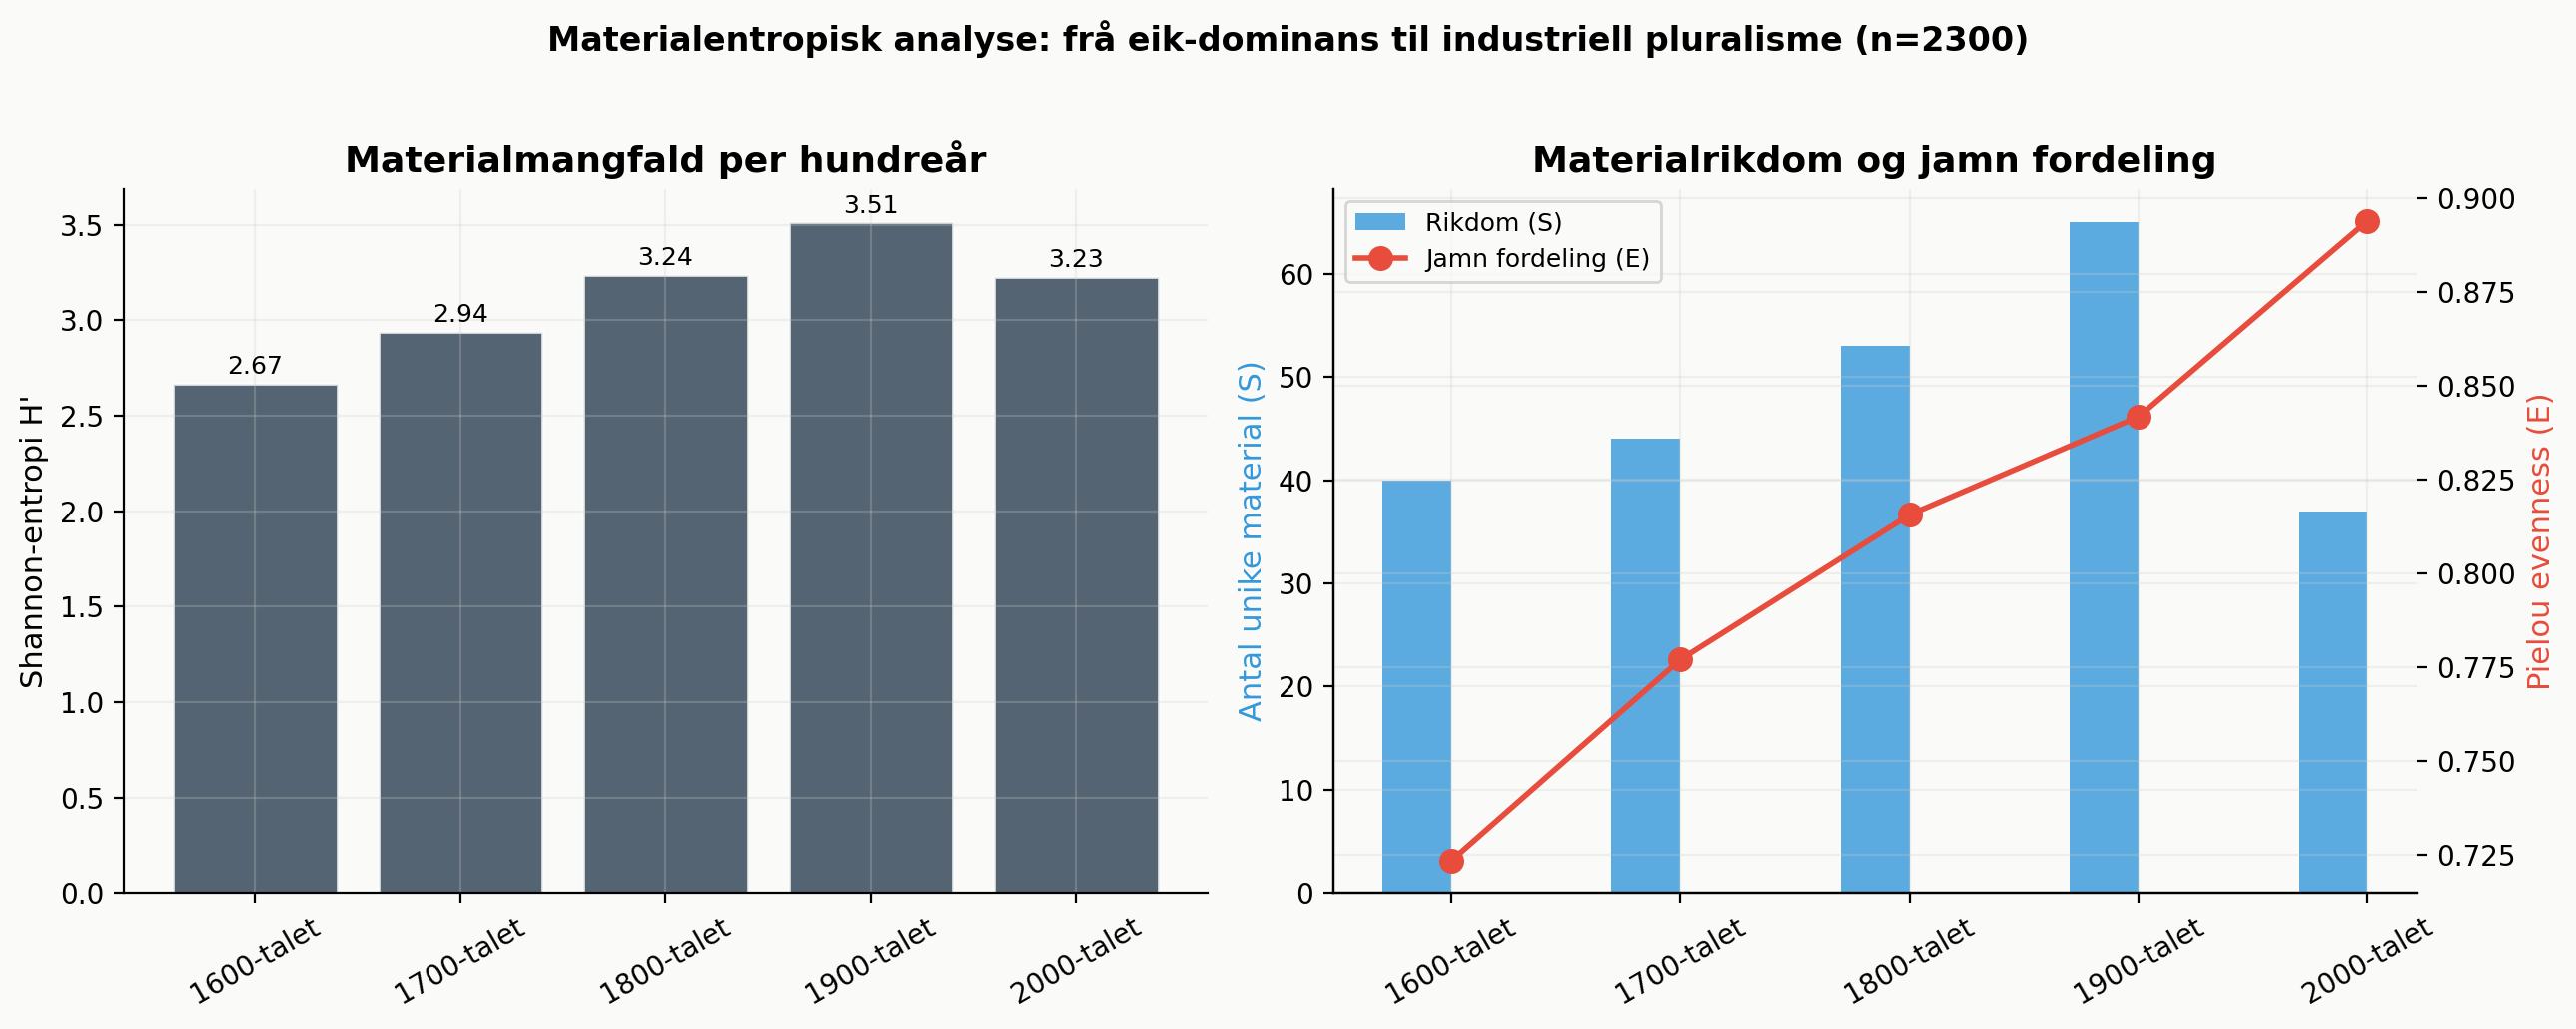
\includegraphics[width=\columnwidth]{07_material_entropy.png}
  \caption{Shannon-entropi ($H'$ i bits) og materialrikdom ($S$) per hundreår.}
  \label{fig:entropi}
\end{figure}

Tabell~\ref{tab:entropy} og figur~\ref{fig:entropi} syner hovudresultata.

\begin{table}[H]
\centering
\caption{Shannon-entropi ($H'$ i bits), tal unike materialar ($S$), og Pielou-jamnheit ($J'$) per hundreår.}
\label{tab:entropy}
\begin{tabular}{@{}lrrrrrr@{}}
\toprule
\textbf{Hundreår} & \textbf{$N$} & \textbf{Førek.} & \textbf{$S$} & \textbf{$H'$} & \textbf{$H'_{\max}$} & \textbf{$J'$} \\
\midrule
1200-talet &     1 &       2 &  2 & 1,00 & 1,00 & 1,00 \\
1500-talet &    14 &      16 &  4 & 1,49 & 2,00 & 0,75 \\
1600-talet &   271 &     514 & 40 & 3,85 & 5,32 & 0,72 \\
1700-talet &   669 &  1\,759 & 44 & 4,24 & 5,46 & 0,78 \\
1800-talet &   510 &  1\,363 & 53 & 4,67 & 5,73 & 0,82 \\
1900-talet &   721 &  1\,705 & 65 & 5,07 & 6,02 & 0,84 \\
2000-talet &    92 &     167 & 37 & 4,66 & 5,21 & 0,89 \\
\bottomrule
\end{tabular}
\end{table}

Dataa avdekkjer tre materialregime:

\textbf{Regime I: Det lokale treregimet (1200--1500).} Bjørk, furu, eik. $H' < 2$ bits. Materialradien er lokal. Gårastolen er prototypen.

\textbf{Regime II: Det koloniale handelsregimet (1600--1800).} 33 nye materialar eksploderer inn på 1600-talet: mahogni, ibenholt, palisander, rotting, silke, messing. Globalt treverk stig frå 0\,\% til 18,9\,\% av alle materialførekomstar (figur~\ref{fig:kategoriar}). Mahogni åleine vert det nest mest brukte materialet i heile databasen (472 førekomstar, 8,5\,\%).

\textbf{Regime III: Det industrielt-syntetiske regimet (1900--2000).} Globalt treverk kollapsar frå 18,9\,\% til 1,2\,\%. Industrielle materialar (stål, kryssfiner, plast) eksploderer frå 0,4\,\% til 32,3\,\%. Utvinningspunktet flyttar seg frå tropisk skog til oljefelt.

\begin{figure}[H]
  \centering
  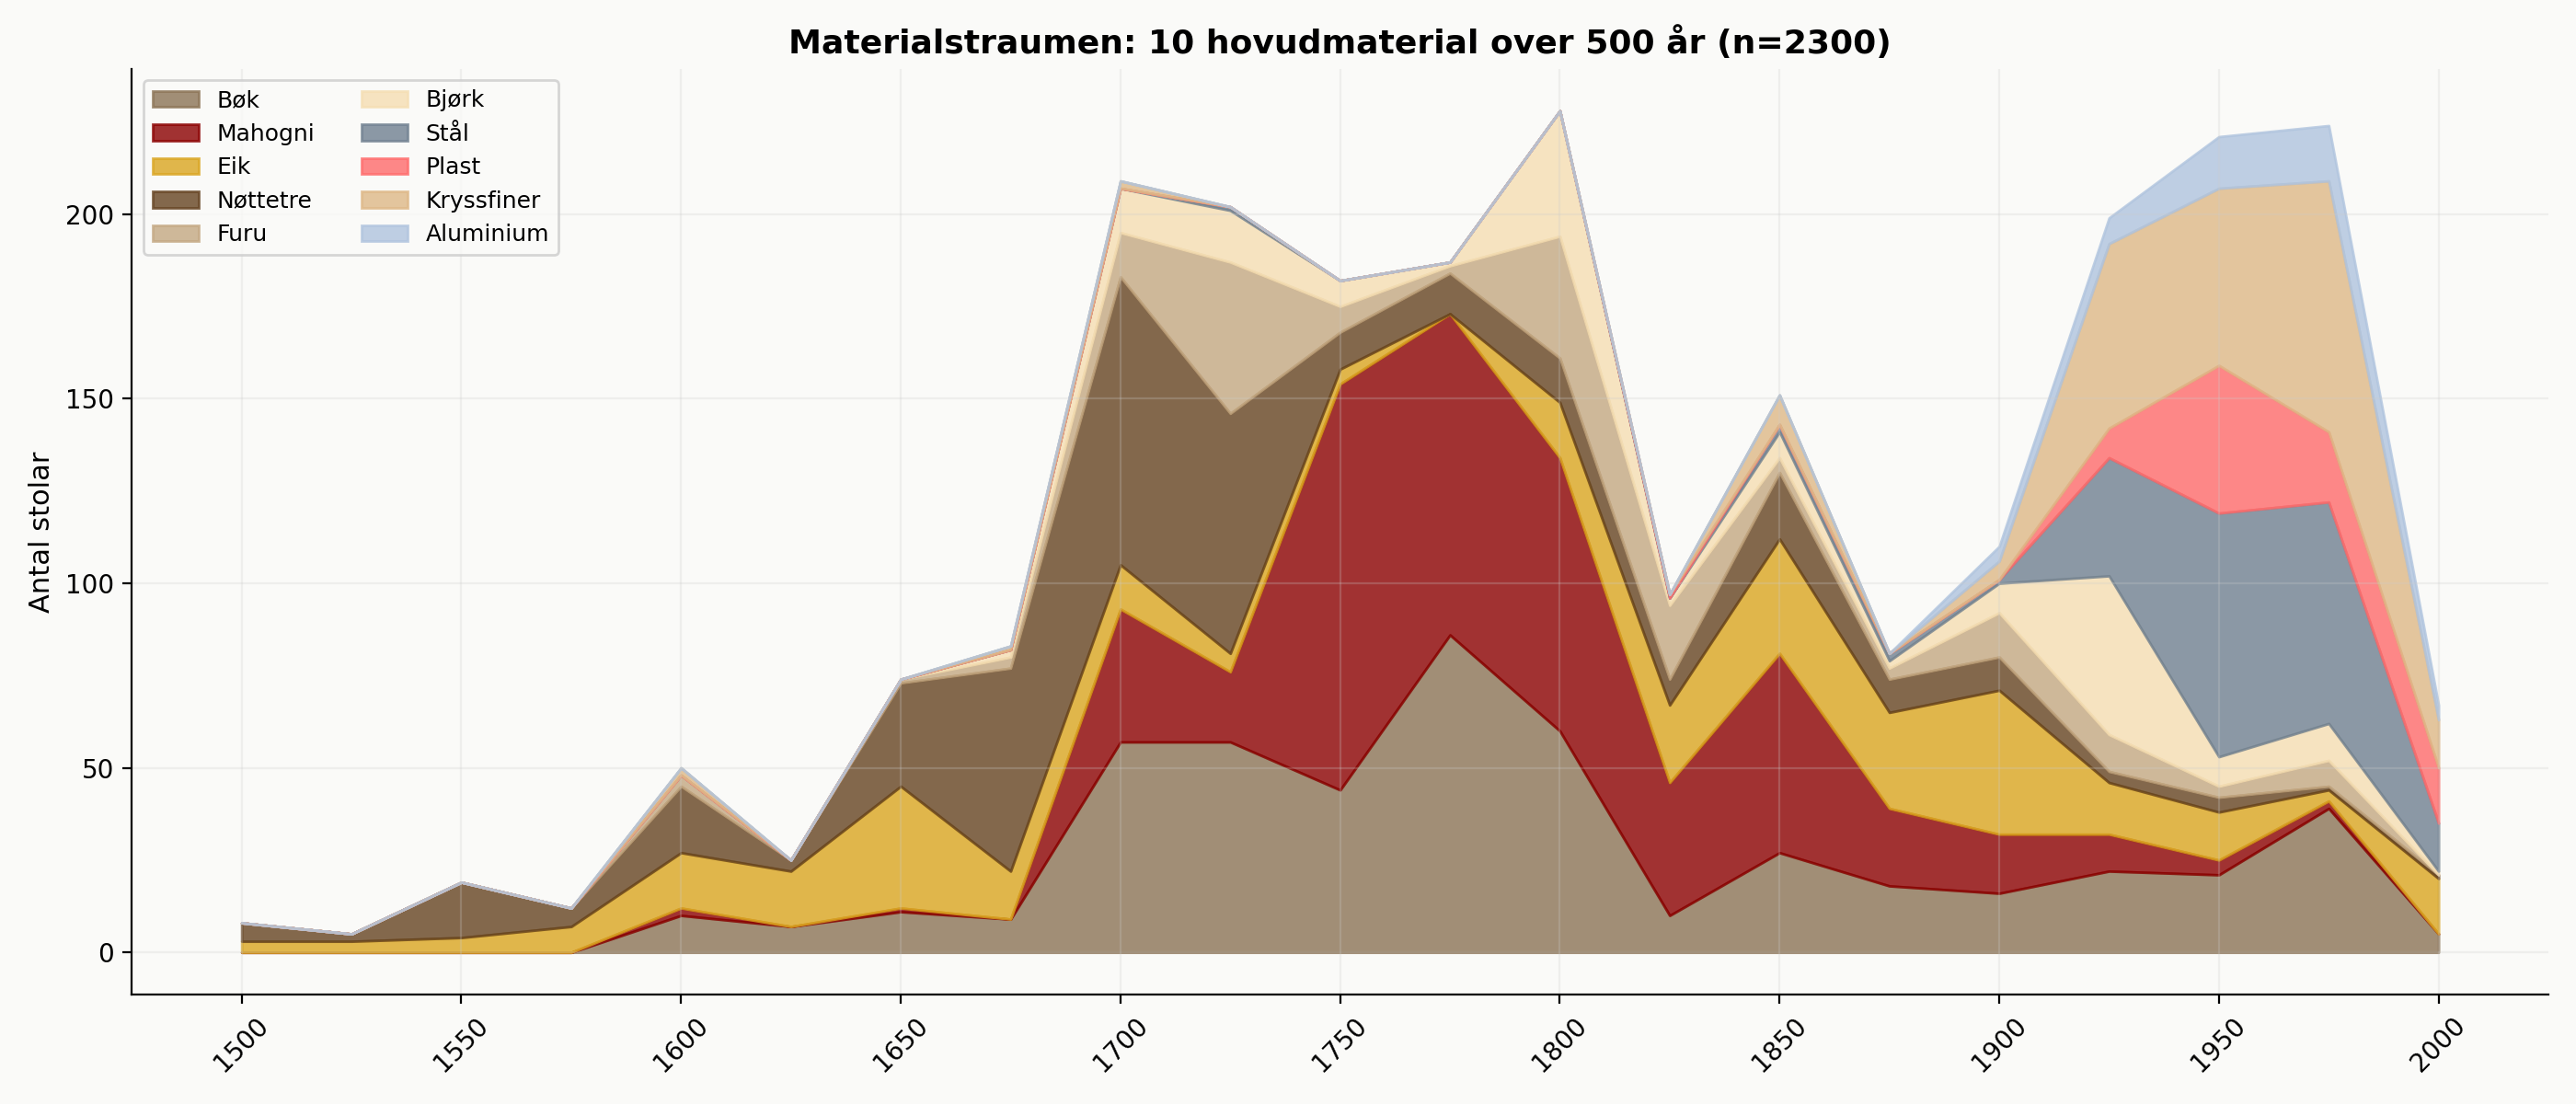
\includegraphics[width=\columnwidth]{01_material_river.png}
  \caption{Tre materialepokar: lokalt (grønt), kolonialt (brunt), industrielt (oransje). Kryssingspunktet mellom kolonialt og industrielt materiale ligg rundt 1875--1900.}
  \label{fig:kategoriar}
\end{figure}


\subsection{NMK og V\&A: sentrum og periferi}

Mahogni-bogen i NMK og V\&A følgjer ulike tidskurver (tabell~\ref{tab:mahogni}). I V\&A toppar mahogni på 1700-talet (17,3\,\% av materialførekomstane); i NMK fyrst på 1800-talet (16,1\,\%). Den koloniale materialstraumen nådde London eit hundreår før han spreidde seg til nordiske periferiar. Noreg er ein \emph{sekundærmottakar} av koloniale materialar: me importerer via London, ikkje direkte fraa Karibia. I \citet{wallerstein2004} sin terminologi okkuperer Noreg ein klassisk semi-perifer posisjon: tilbydar av raavarer (deal-tommar) til den britiske produksjonskjernen, samstundes mottakar av ferdige varer og designmonster. Danmark-Noreg var direkte involvert i karibisk kolonialisme gjennom dei vestindiske oyane (St. Thomas, St. John, St. Croix), med om lag 110\,000 slavar transporterte paa danske skip fraa 1660-aara til 1803. Mahogni-stolen i Nasjonalmuseet er ikkje berre eit spor av britisk imperialisme; han er eit spor av \emph{dansk-norsk} kolonialisme.

Produksjonsstatistikken forsterkar dette biletet. Av dei 134 mahogni-stolane i NMK med registrert produksjonsstad kjem 37 frå Storbritannia, 31 frå Noreg og 31 frå Danmark. Med andre ord: nesten ein tredel av dei norske museumsinstalasjonane med mahogni er \emph{importerte ferdige} frå den koloniale metropolen. Dei resterande er norskproduserte, men med importert materiale. Stolen er kolonial uansett om det er materialet eller heile gjenstanden som har reist over havet.

Stilmessig dominerer \textbf{empire} (36 stolar) blant mahogni-stolane i NMK, følgd av \textbf{historisme} (21) og \textbf{hepplewhite} (18). Empire-stilen, med sine stramme nyklassisistiske liner og tunge mahognifasadar, er i denne forstand ikkje berre ein estetisk kategori: han er ein \emph{kolonial materialkode}.

\begin{table}[H]
\centering
\caption{Mahogni som prosent av alle materialførekomstar, per museum.}
\label{tab:mahogni}
\begin{tabular}{@{}lrrr@{}}
\toprule
\textbf{Hundreår} & \textbf{Samla} & \textbf{NMK} & \textbf{V\&A} \\
\midrule
1600-talet &  0,8\,\% &  1,3\,\% &  0,6\,\% \\
1700-talet & 14,3\,\% &  7,2\,\% & 17,3\,\% \\
1800-talet & 13,6\,\% & 16,1\,\% & 11,8\,\% \\
1900-talet &  1,9\,\% &  2,5\,\% &  1,7\,\% \\
\bottomrule
\end{tabular}
\end{table}

\textbf{Jaccard-avstanden} mellom dei to musea si materialpalett (figur~\ref{fig:jaccard}) fell frå 1,0 (1400-talet) til 0,32 (1900-talet): globaliseringa homogeniserer materialtilgangen.

\begin{figure}[H]
  \centering
  
\includegraphics[width=\columnwidth]{fig4_jaccard.pdf}
  \caption{Jaccard-avstand mellom NMK- og V\&A-materialpalettar. Konvergensen demonstrerer globaliseringa si materialhomogenisering.}
  \label{fig:jaccard}
\end{figure}


\subsection{Materiell dobbeltheit}

\begin{figure}[H]
  \centering
  
\includegraphics[width=\columnwidth]{teikn_dobbeltheit_prosess.png}
  \caption{Prosessen med materiell dobbeltheit: (1) lokal furukjerne, (2) paaforing av mahognifiner, (3) beising og polering for mahogni-uttrykk. Skaping av kolonialsimulakring.}
  \label{fig:dobbeltheit_prosess}
\end{figure}

\begin{figure}[H]
  \centering
  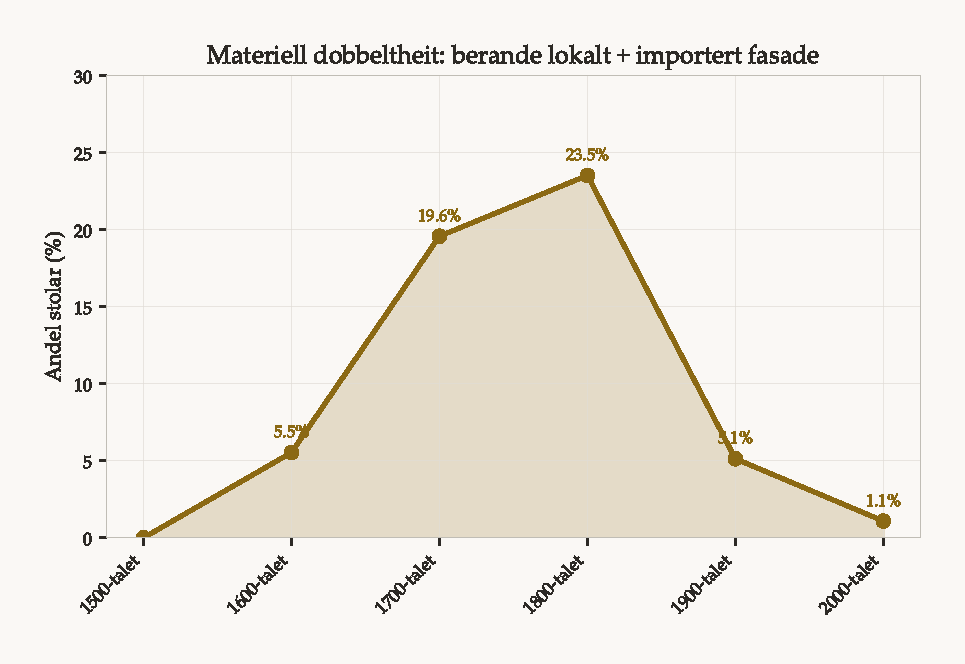
\includegraphics[width=\columnwidth]{fig10_dobbeltheit.pdf}
  \caption{Materiell dobbeltheit over tid: andel stolar med baade lokalt berande tre og importert fasademateriale. Toppar 23,5\,\% paa 1800-talet.}
  \label{fig:dobbeltheit}
\end{figure}

Me kallar det \textbf{materiell dobbeltheit} når den berande kjernen er bygd i lokalt virke (bjørk, furu, bøk) medan den ytre fasaden er trekt i importert edelt materiale (mahogni, silke, palisander). Fenomenet toppar med 23,5\,\% av stolane på 1800-talet (figur~\ref{fig:dobbeltheit}). Dobbeltheitskurva speglar mahogniens boge nesten perfekt: ho veks med imperiet og forsvinn med det.

Eit talande eksempel er \textbf{OK-10888-serien}: tolv empirestolar frå om lag 1820, produserte i Danmark, alle med same materialresept. Museumskatalogen beskriv dei som \emph{``fernissert cubamahogni finert på bøk og eik med marketeridekor i buksbom, hestehårstrekk''}. Konstruksjonen avslører eit presist hierarki: den berande ramma av europeisk \emph{bøk} og \emph{eik} er usynleg under eit tynt lag av \emph{cubamahogni}, importert frå Karibia via danske og britiske handelsnettverk. Innlagt \emph{buksbom}-dekor markerer presisjon og prestisje; \emph{hestetagl} frå europeiske leverandørkjeder fyller polstringa. Seks materialar, tre kjelder: nordisk skog (bøk, eik), karibisk plantasje (cubamahogni), europeisk handverksnettverk (buksbom, hestetagl). Den usynlege bøka ber vekta; den synlege mahognien ber prestisjen. Konstruksjonen er eit \emph{materialisert makthierarki}.

Eit endå meir ekstravagant eksempel er \textbf{OK-07355} frå byrjinga av 1800-talet: ein nyklassisistisk stol med \emph{beiset og lakkert cubamahognifiner med ibenholt, relieffskjering og forgylt bronsedekor}. Her er to koloniale materialar til stades samstundes: \emph{cubamahogni} frå Karibia og \emph{ibenholt} frå Søraust-Asia, bundne saman av europeisk \emph{bronse}. Den berande ramma er lokal \emph{bjørk}, \emph{bøk} og \emph{furu}. Éin stol, seks materialar, tre kontinent, eitt maktsystem.

Når industrielle materialar tek over på 1900-talet, vert dobbeltheit overflødig. Etter 1875 stig \emph{eik} tilbake som dominerande materiale i NMK (34 førekomstar i 1875--1950), og den koloniale fasaden vert erstatta av eit nasjonalromantisk og seinare modernistisk materialuttrykk. Plast og stål treng ikkje kamuflerast; dei er sjølvtilstrekkelege.


% ================================================================
\section{Diskusjon}

\subsection{Mahogni som kolonialt termometer}

Mahogniens boge (figur~\ref{fig:mahogni}) kan lesast som eit \textbf{kolonialt termometer}: prosentdelen av stolar med mahogni er ein direkte indikator på Noreg sin integrasjon i det transatlantiske handelsnettet. Når bogen stig, stig den koloniale tilkoplinga; når han fell, fell ho.

Kulminasjonspunktet ved 100\,\% i 1825--1849 er ikkje berre eit statistisk kuriosum. Det er eit symptom på kva \citet{wallerstein2004} kalla eit \textbf{verdsystem} der perifere handverkarar er fullstendig avhengige av sentrum sine materialstraumar. Den norske snikkaren i 1830 har \emph{ikkje val}: han lagar stolen av mahogni fordi det er det materialet som er tilgjengeleg, prissett og estetisk forventa. Stolen er ikkje kolonial fordi snikkaren vel det; han er kolonial fordi \emph{materiallandskapet} er kolonialt. Mekanismen er det som i evolusjonaer kulturteori vert kalla \textbf{prestisjebias}: menneske kopierer former fraa hoegstatusindivid. Mahogni-stolen er ikkje vald fordi han er funksjonelt overlegen; han er vald fordi han er assosiasjonelt attraktiv: han signaliserer tilknyting til det imperiale sentrumet. Prestisjebias forklarer kvifor mahogni-monopolet er saa totalt: det er ikkje nok aa ha mahogni; ein \emph{maa} ha mahogni for aa signalisere status. Materialet vert ein sosial kode, ikkje eit konstruksjonsval.

\subsection{Utforsking og utnytting}

Mahogniens boge illustrerer eit mønster som \citet{kauffman1993} og \citet{sutton2018} har formalisert som avveginga mellom \textbf{utforsking} (exploration) og \textbf{utnytting} (exploitation). I utforskingsfasar prøver aktørar mange materialar og konvergerer ikkje; entropien stig. I utnyttingsfasar konvergerer dei rundt eit funne optimum; entropien fell.

\begin{figure}[H]
  \centering
  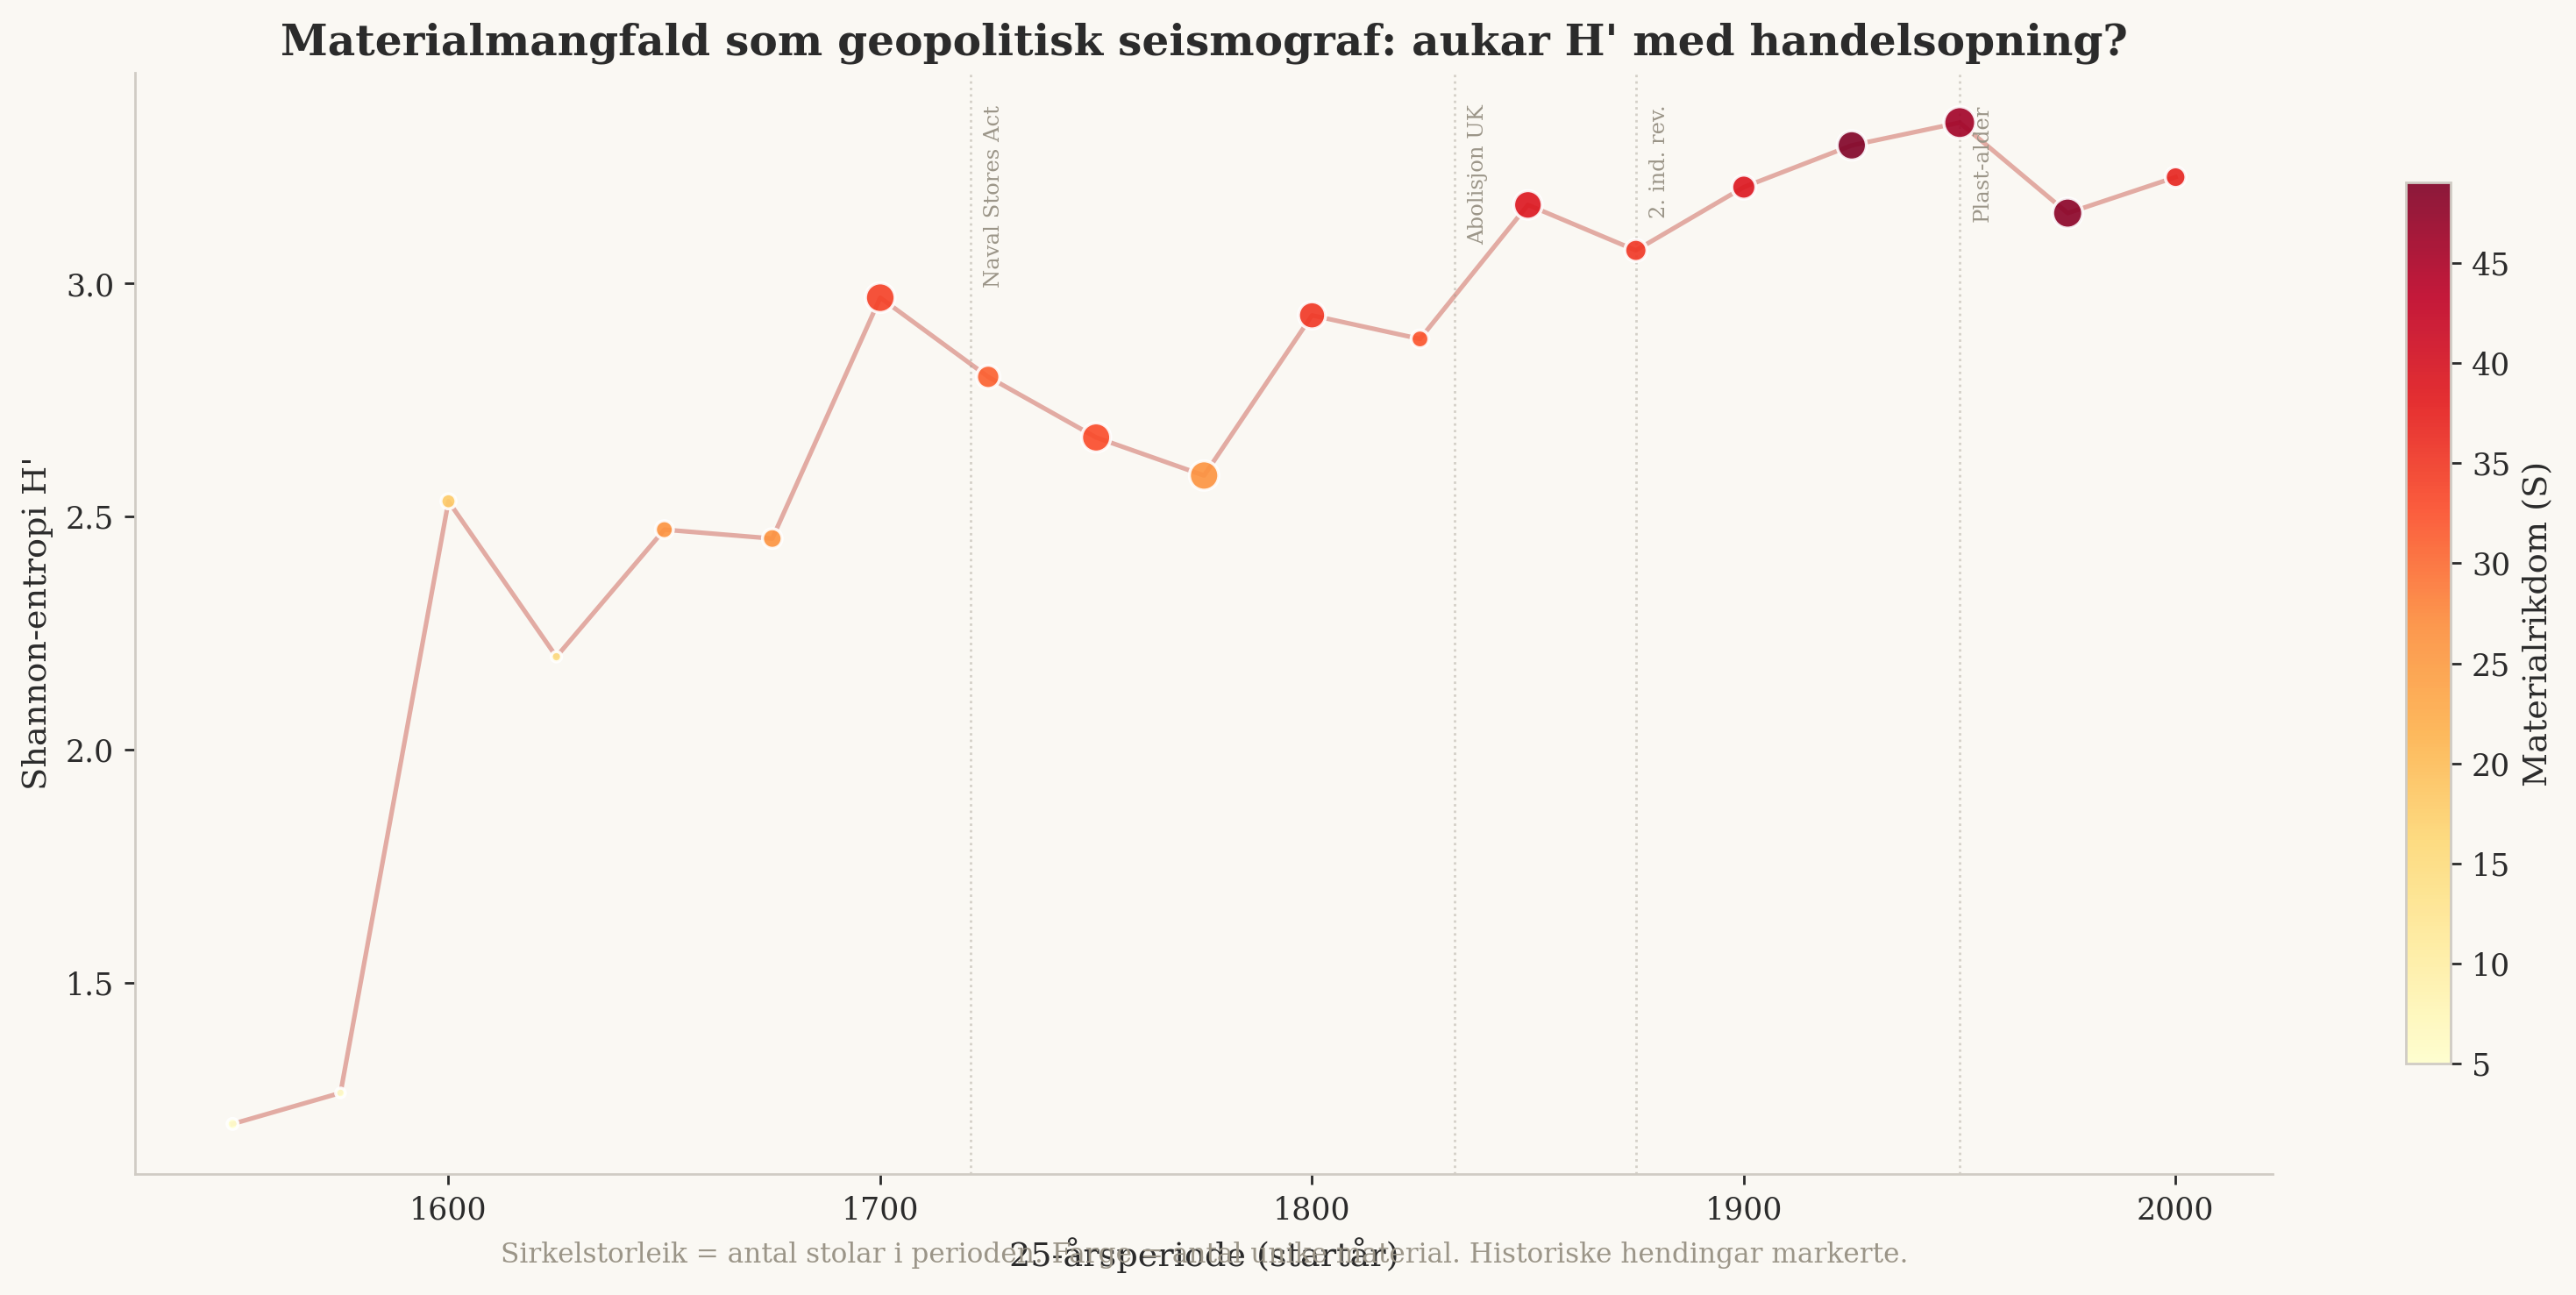
\includegraphics[width=\columnwidth]{02_entropy_trade_proxy.png}
  \caption{Rullande 50-aarsentropi: utforskingsfasar (stigande $H'$) og utnyttingsfasar (fallande $H'$). Mahogni-monopolet rundt 1750--1800 er tydeleg som eit dip.}
  \label{fig:expl}
\end{figure}

Mahogni-monopolet i NMK (1800--1849) er den tydelegaste \emph{utnyttingsfasen} i heile databasen: eit einaste materiale har vorte identifisert som den beste tilgjengelege løysinga (estetisk, økonomisk, statusmessig), og heile produksjonen konvergerer rundt det. Når tilgangen endrar seg (avskoging, industrialisering, endra handelsruter), vert det naudsynt med ny utforsking: eik, furu og seinare stål og plast konkurrerer om dei ledige nissjane.

Denne oscillasjonen mellom utforsking og utnytting svarar til det \citet{eldredge1972} kalla \textbf{punctuated equilibrium} i biologisk evolusjon: lange periodar med stasis (mahogni-monopolet) avbrotne av raske brot (industrialiseringa). Materialhistoria er ikkje lineært framsteg; ho er ein serie av konsolideringar og omveltingar.

\subsection{Den post-koloniale tilbakekomsten av lokalt tre}

Etter mahogniens fall opnar det seg eit materialt vakuum i norsk stoldesign. Tiårsdata avdekkjer ein presis materialsuksesjon:

\begin{enumerate}
  \item \textbf{1880-talet}: Eik tek over (38,6\,\% av NMK-stolar). Nasjonalromantikken rehabiliterer lokalt trevirke.
  \item \textbf{1920-talet}: Stål debuterer som dominerande materiale (23\,\%). Bauhaus og internasjonal modernisme.
  \item \textbf{1930-talet}: Bjørk eksploderer til 29,6\,\%, kryssfiner til 24,5\,\%. Aalto-effekten: dampbøygd finsk bjørk vert det nye paradigmet.
  \item \textbf{1940-talet}: Kryssfiner dominerer (38,1\,\%). Eames-paret sin laminerte teknologi.
  \item \textbf{1950-talet}: Stål (45,2\,\%) og glasfiber (25,8\,\%). Den industrielle materialalderen er fullt realisert.
\end{enumerate}

\begin{figure}[H]
  \centering
  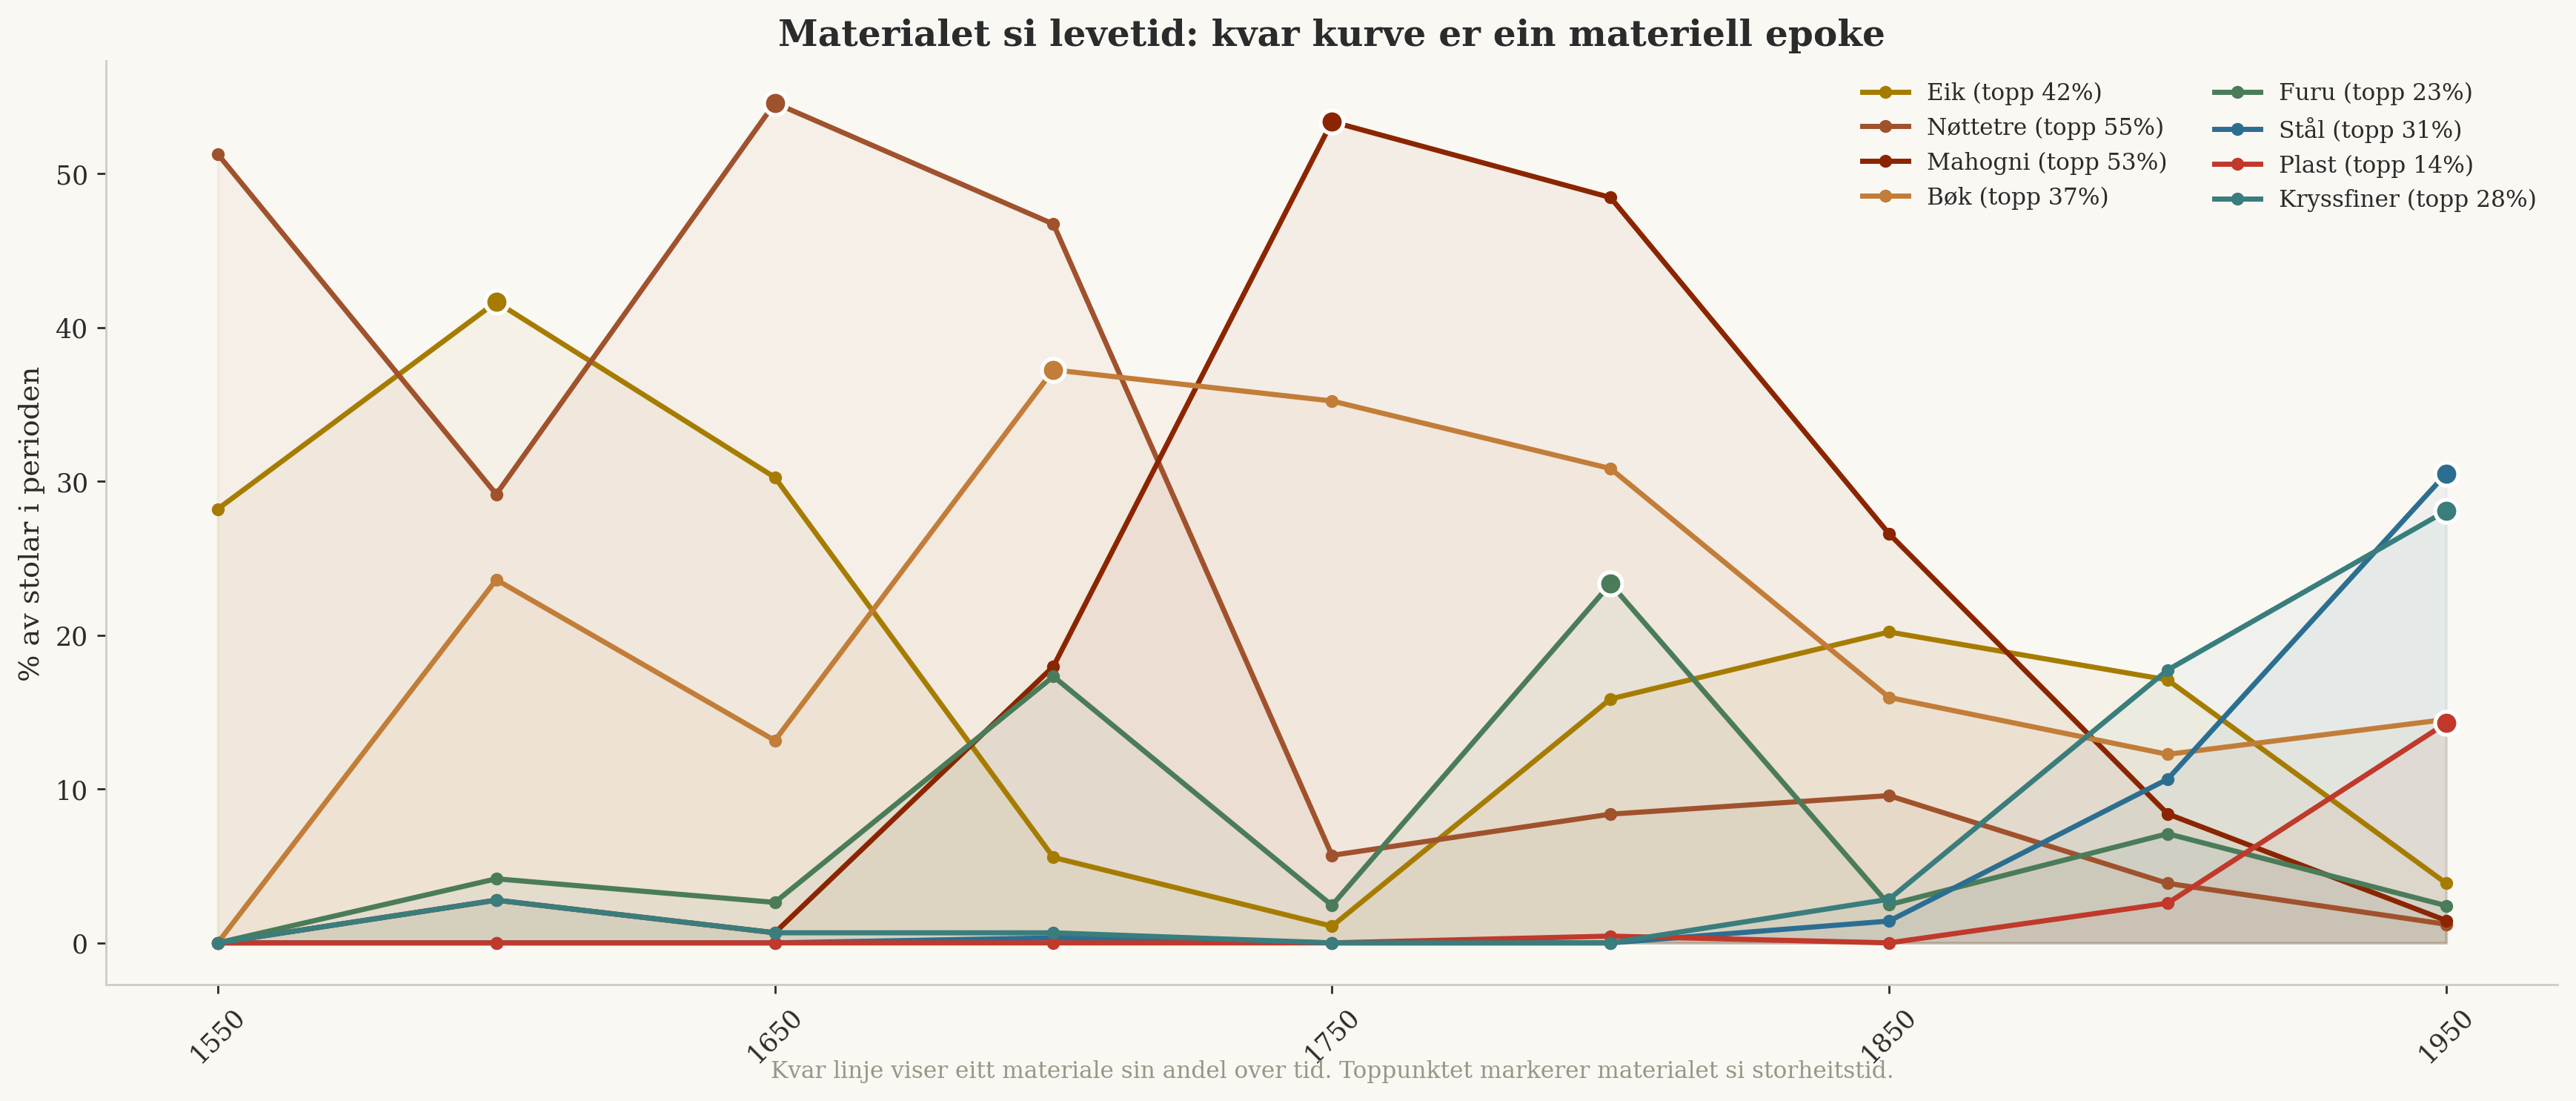
\includegraphics[width=\columnwidth]{11_material_lifespans.png}
  \caption{Materialsuksesjon i Nasjonalmuseet, 1700--2020. Mahogni (moerkt brunt) dominerer 1750--1850, deretter tek eik, staal, bjork og kryssfiner over.}
  \label{fig:succession}
\end{figure}

Denne suksesjonen er ikkje tilfeldig. Kvart materiale krev ein ny teknikk som igjen opnar nye regionar i formrommet: stål krev sveising og røyrbøying; bjørk krev dampbøying og laminering; glasfiber krev støyping. Materialsuksesjonen er samstundes ein teknikksuksesjon og ein formsuksesjon.

Denne tilbakevendinga til lokalt treverk i 1880-åra er ikkje tilfeldig: ho fell saman med den norske nasjonalromantikken, der \emph{det norske} (dragestil, stavkyrkjeornament, lokalt trevirke) vart estetisk rehabilitert som motreaksjon til det importerte og kosmopolitiske.

Kontrasten mellom to samtidige designarar krystalliserer dette: \textbf{Lars Kinsarvik} (2 stolar i databasen, begge i ``skoren og måla furu'') og \textbf{Thomas Chippendale} (12 stolar, 67\,\% mahogni, ``skoren mahogni''). Begge nyttar skjereteknikk; begge arbeider med tre. Men materialet er diametralt motsett: Kinsarvik sitt lokale furu vs. Chippendale si karibiske mahogni. Kinsarvik sin stol er eit nasjonalromantisk manifest; Chippendale sin er eit kolonialt manifest. Same teknikk, same funksjon, motsett geopolitisk posisjon.

Eit talande uttrykk for denne motreaksjonen er \textbf{stolen frå Eventyrværelset} (OK-1995-0109), datert 1897: ein armstol i \emph{utskoren og bemalt furu}. Ikkje eit gram importert materiale. Furu, det mest lokale av alle norske treslag, vert her opphøgd til kunstnarleg uttrykksmiddel gjennom jugendstilen sin ornamentelle skjereteknikk. Eventyrværelset-stolen er mahogniens antitese: der mahognistolen skjuler lokalt tre bak ein importert fasade, \emph{feirer} denne stolen det lokale treet som estetisk mål i seg sjølv.

\subsection{Materialradius: kvantifisering av geografisk rekkjevidd}

\begin{figure}[H]
  \centering
  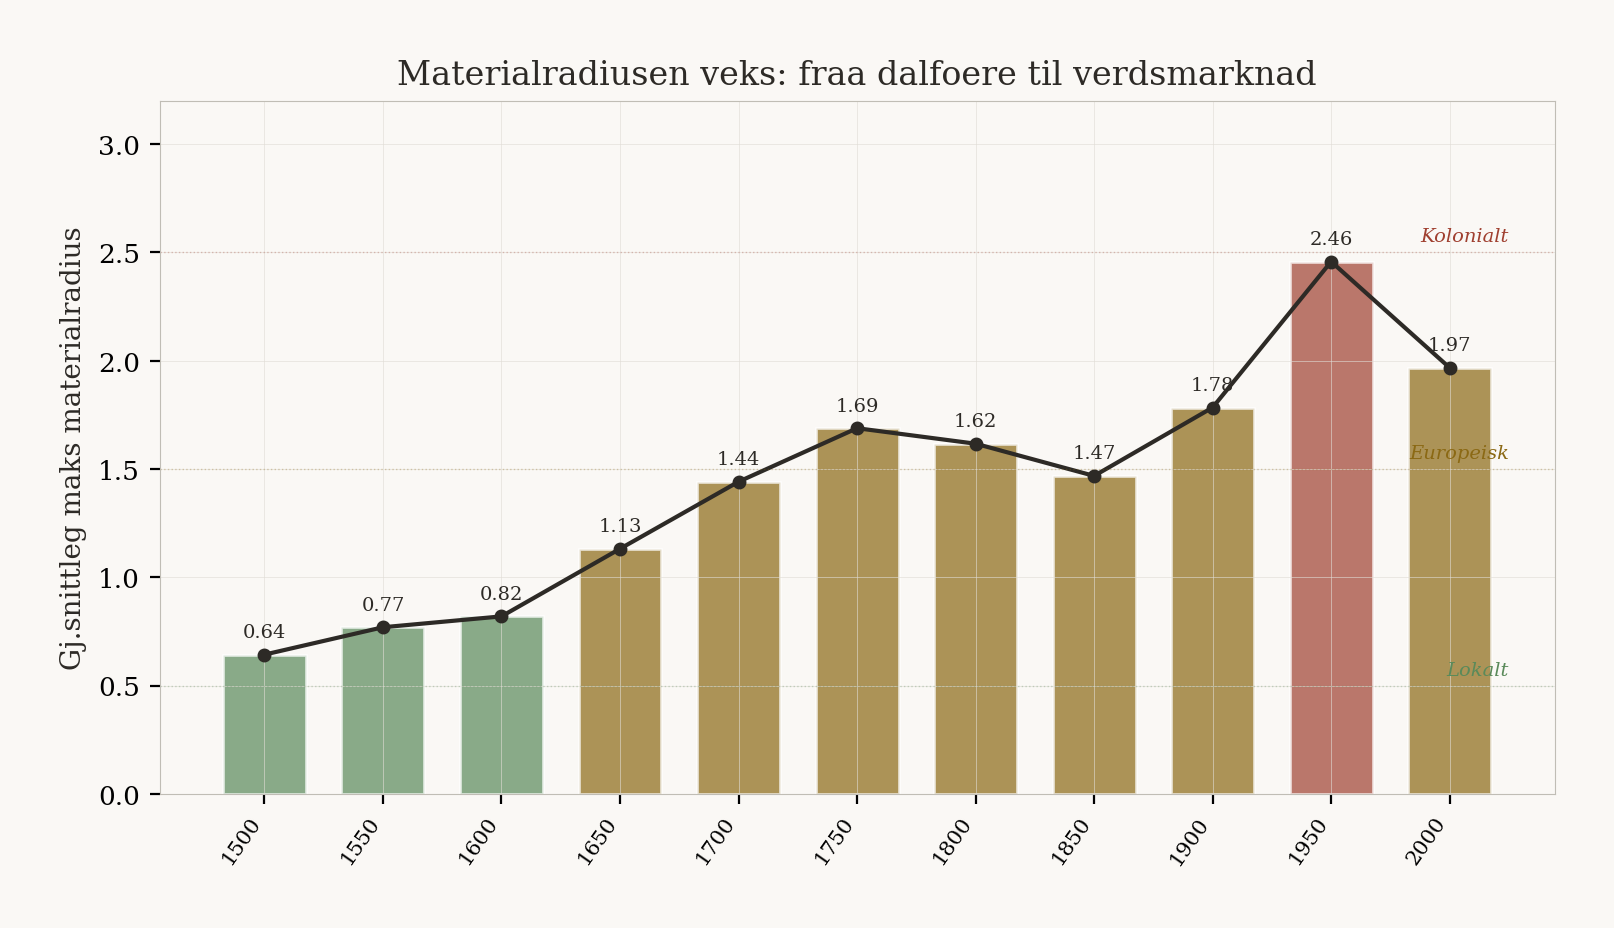
\includegraphics[width=\columnwidth]{fig24_materialradius.png}
  \caption{Materialradiusen veks: gjennomsnittleg maksimal geografisk rekkjevidd per stol over tid. Fraa lokalt dalfoere (0) til globalt industrielt nettverk (3).}
  \label{fig:radius}
\end{figure}

Me kan kvantifisere kor langt materiala reiser ved å tilordne kvar materialkategori ein \textbf{radius}: 0 (lokalt, $<$100 km), 1 (europeisk, 100--2\,000 km), 2 (kolonialt/interkontinentalt, $>$5\,000 km), og 3 (industrielt, globalt men abstrahert frå geografi). Den gjennomsnittlege maksimale materialradiusen per stol stig frå 0,64 (1500-talet) til 2,46 (1950--1999). Kvar stol sitt materialnettverk strekk seg bokstavleg talt lenger og lenger over jordkloden. Gårastolen (1280) har ein materialradius på null: begge materiala veks innanfor gangavstand. OK-10888 (1820) har ein radius på 2: cubamahogni frå Karibia. Ein plastkrakk frå 2000-talet har ein radius på 3: polypropylen frå ein petrokjemisk terminal som kan ligge kvar som helst.

\subsection{Ergonomisk ratio: stolen mistar ryggen}

\begin{figure}[H]
  \centering
  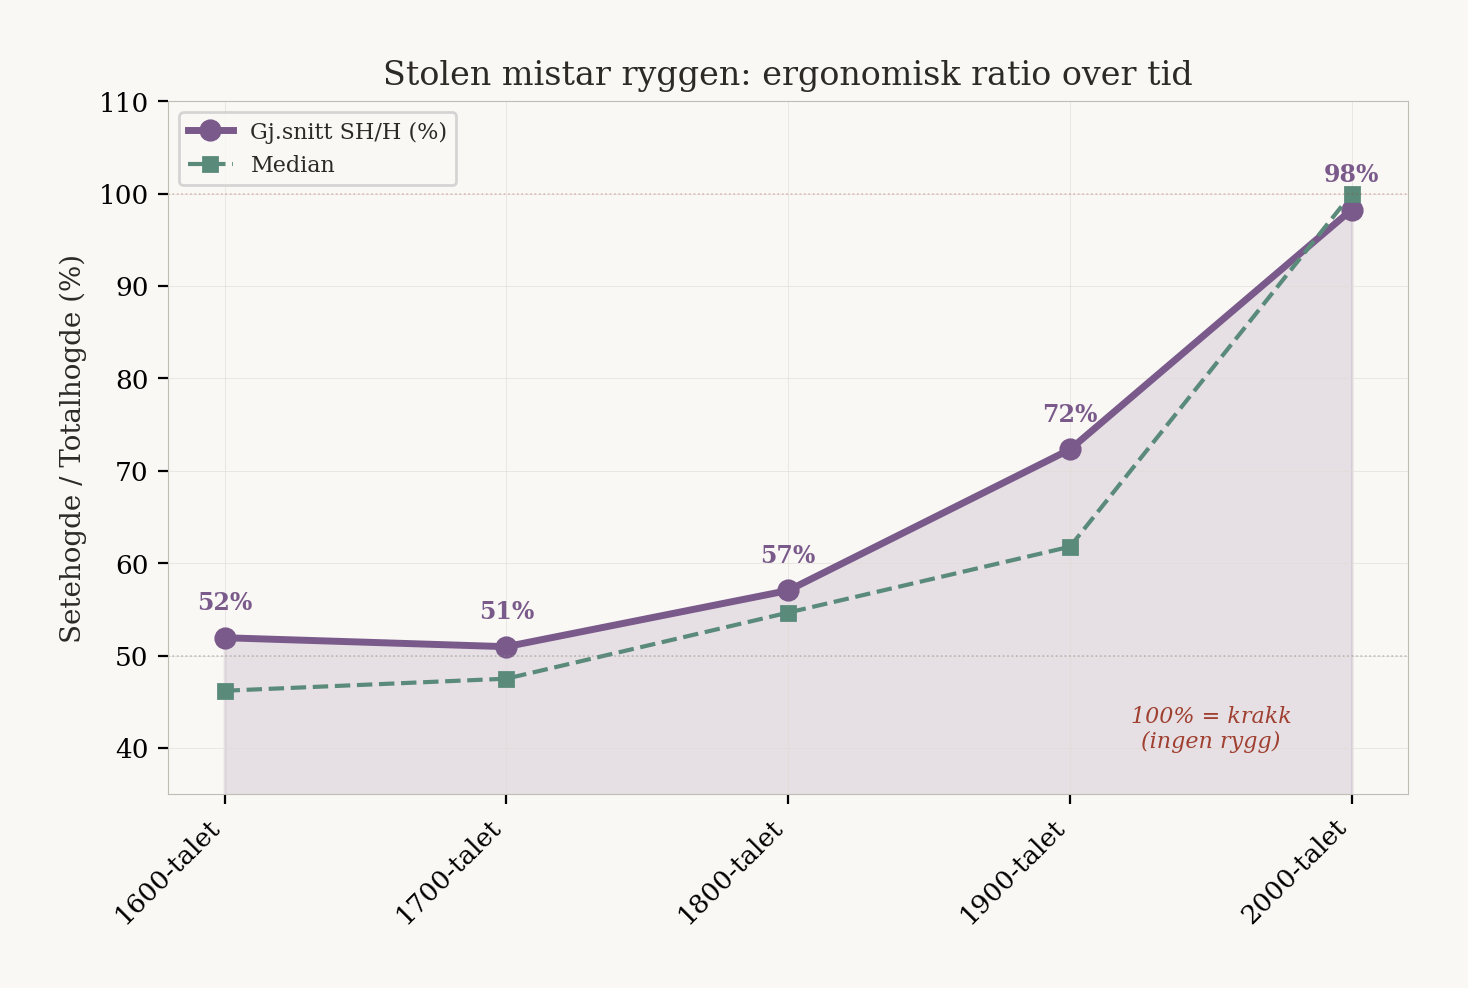
\includegraphics[width=\columnwidth]{fig23_ergonomisk_ratio.png}
  \caption{Stolen mistar ryggen: setehogde som prosent av totalhogde stig fraa 52\,\% til 98\,\%.}
  \label{fig:ergonomisk}
\end{figure}

Eit overraskande bifunn frå dimensjonsanalysen er at forholdet mellom setehøgde og totalhøgde (SH/H) endrar seg dramatisk over tid: frå 52\,\% på 1600-talet til 72\,\% på 1900-talet og 98\,\% på 2000-talet. Stolen er bokstavleg talt i ferd med å miste ryggen. Barokkstolen har ein rygg som utgjer nesten halvparten av den totale høgda; den moderne stolen har knapt rygg i det heile. Denne overgangen reflekterer ikkje ein ergonomisk forbetring (ryggar er framleis nyttige), men ein \emph{stilistisk og materiell} endring: nye materialar (stål, plast) mogeleggjer sjølvberande setkonstruksjonar som ikkje treng ein tradisjonell stolperamme.

\subsection{Material follows access}

\citet{sullivan1896} sitt aksiom \emph{form follows function} impliserer at funksjonen bestemmer materialvalet. Men funksjonen til ein stol (å sitje på) har ikkje endra seg sidan 1280. Likevel har materialpaletten eksplodert frå 2 til 65 kategoriar, og mahogni har gått frå null til monopol og tilbake. Det er ikkje funksjonen som driv materialvalet; det er \emph{tilgang}.

\begin{quote}
\textbf{Material follows access:} Materialvalet i ein gjenstand reflekterer ikkje primært funksjonen hans, men det historisk betinga \emph{tilgangsrommet}: kva tre som veks i nærleiken, kva hamner som er opne, kva koloniale forsyningskjeder som eksisterer, og kva industrielle prosessar som er tilgjengelege.
\end{quote}

Denne formuleringa er empirisk testbar. Dersom materialet følgde funksjonen, ville me forvente låg entropi og stabil materialpalett over tid (funksjonen er jo konstant). I staden observerer me mahogniens boge: ein dramatisk svingande kurve driven av geopolitiske, ikkje funksjonelle, krefter. Materialet følgjer ikkje funksjonen; materialet følgjer makta.

I rammeverket fraa \emph{form(al) logikk}: funksjonen definerer eit \emph{delrom} i morphospace, ikkje eit punkt. For ein stol er dette delrommet enormt: alle konfigurasjonar som kan bere ein sitjande kropp. Innanfor delrommet er det seleksjonstrykk (materiale, teknologi, geografi, kultur) som vel posisjon. Funksjonen seier: ``det maa finnast ei flate aa sitje paa.'' Utover dette teier ho. Mahogniens boge, materialentropiens stigning, den materielle dobbeltheita: alt dette er variasjon \emph{innanfor} det funksjonelle delrommet, driven av krefter funksjonen ikkje kan forklare.

\subsection{Historiske knutepunkt}

\begin{figure}[H]
  \centering
  
\includegraphics[width=\columnwidth]{fig25_historiske_knutepunkt.png}
  \caption{Shannon-entropi ved historiske knutepunkt. Kvart geopolitisk og teknologisk sjokk endrar materiallandskapet maelbart.}
  \label{fig:knutepunkt}
\end{figure}

Materialentropien ved historiske knutepunkt (figur~\ref{fig:knutepunkt}) avdekkjer ein direkte korrelasjon mellom geopolitiske hendingar og materiell kompleksitet. Ved sjuårskrigen (1750) dominerer mahogni med 100 førekomstar, og entropien er $H' = 4{,}07$ bits: den koloniale utnyttingsfasen komprimerer mangfaldet. Ved Bauhaus (1925) har bjørk og kryssfiner teke over, og entropien er $H' = 4{,}74$ bits: det industrielle regimet utvidar paletten. \subsection{1500-1600: den storste materialomveltinga}

Jaccard-avstand mellom paafolgande hundreaar avdekkjer at overgangen fraa 1500- til 1600-talet er den absolutt storste materialomveltinga i heile datamaterialet: $d_J = 0{,}927$. Berre 3 av 41 materialar er delte; 37 er \emph{nye}. Denne eine overgangen, driven av den europeiske handelsekspansjonen, innforer nesten heile det koloniale materialrepertoaret i eitt jafs. Til samanlikning er overgangen 1700--1800 langt mildare ($d_J = 0{,}30$): etter den initiale eksplosjonen stabiliserer materialpaletten seg. Den nest storste omveltinga er 1900--2000 ($d_J = 0{,}48$), men her er det ikkje nye materialar som driv endringa, men \emph{tap}: 30 materialar forsvinn. Materialverda krympar for fyrste gong.

\subsection{Tidsforseinking: globaliseringa sin akselerasjon}

Tidsforseinkinga mellom V\&A (London) og NMK (Oslo) for nye materialar gjev eit direkte maal paa globaliseringa sin akselerasjon: staal kjem 184 aar seinare til Noreg enn til Storbritannia; plast 93 aar; aluminium 57 aar; glasfiber 38 aar. Forseinkinga \emph{minkar eksponentielt}. Verda vert mindre, og materiallandskapet vert globalt. Denne akselerasjonen korresponderer med Jaccard-konvergensen (figur~\ref{fig:jaccard}): dei to musea sine materialpalettar naermar seg kvarandre fordi nye materialar spreiier seg raskare.

Materialhistorie og geopolitisk historie er ikkje parallelle disiplinar; dei er \emph{same disiplin} sett frå ulike vinklar.

\subsection{Materialsuksesjon: kva erstattar kva?}

Ein 50-aarsperiode-analyse avdekkjer dei eksakte materialsuksesjonane. Den storste einskild-endringa i heile tidsserien er \textbf{mahogni +17 prosentpoeng} i perioden 1700--1750, samstundes som nøttetre fell med 13 prosentpoeng. Mahogni erstattar ikkje berre nøttetre som favorittmateriale; ho \emph{utkonkurrerer} det. I perioden 1850--1900 kjem den industrielle motoffensiven: staal stig med 4 prosentpoeng, kryssfiner med 6, medan mahogni fell med 8. I 1900--1950 akselererer industrialiseringa: staal +8, plast +5, eik -6. Kvar 50-aarsperiode har sine vinnarar og taparar, og tabellen over suksesjonspar er eit komprimert portrett av teknologisk og geopolitisk endring.

\subsection{Materiell demokratisering}

\begin{figure}[H]
  \centering
  
\includegraphics[width=\columnwidth]{fig26_demokratisering.png}
  \caption{Materiell demokratisering: kvar dominerer sitt hundreaar. Mahogni topper 1750, staal 1950, kryssfiner 1980.}
  \label{fig:demokratisering}
\end{figure}

Figur~\ref{fig:demokratisering} syner korleis ulike materialar dominerer sine epokar: mahogni toppar i 1750 (kolonialt monopol), stål i 1950 (industriell rasjonalisme), kryssfiner i 1980 (laminert demokrati). Kvart materiale si kurve er ein miniatyr-biografi: fødsel, vekst, dominans, tilbaketrekking. Materialverda er ikkje statisk; ho er eit dynamisk økosystem av konkurrerande substrat.

\subsection{Materiell halveringstid}

Me kan definere \textbf{materiell halveringstid} som tida det tek frå eit materiale sin toppperiode til andelen er halvert. Denne metrikken avslører ulike materialdynamikkar:

\begin{table}[H]
\centering
\caption{Materiell halveringstid: kor raskt kollapsar dominansen?}
\label{tab:halflife}
\begin{tabular}{@{}lrrr@{}}
\toprule
\textbf{Materiale} & \textbf{Topp (tiaar)} & \textbf{Topp $n$} & \textbf{Halveringstid} \\
\midrule
Mahogni & 1750 & 68 & $\sim$10 aar \\
Nøttetre & 1730 & 46 & $\sim$10 aar \\
Plast & 1960 & 21 & $\sim$10 aar \\
Staal & 1950 & 38 & $\sim$20 aar \\
Kryssfiner & 1980 & 39 & $\sim$20 aar \\
Bøk & 1780 & 48 & $\sim$30 aar \\
\bottomrule
\end{tabular}
\end{table}

Koloniale og industrielle materialar har kort halveringstid (10--20 aar): dei kjem bratt og forsvinn bratt. Europeiske tradisjonelle materialar (bøk) har lengre halveringstid (30 aar): dei er meir integrerte i handverkspraksis og fell langsamt. Materialmonopol er inherent ustabile: jo brattare stiginga, jo brattare fallet. Mahogni sin halveringstid på 10 aar (fraa toppen i 1750) kontrasterer med bøk sin halveringstid på 30 aar: det lokale materialet held seg lenger fordi det er integrert i handverkspraksis, ikkje avhengig av koloniale forsyningskjeder.

\subsection{Simpson-diversitet: ein uavhengig stadfestring}

For aa stadfeste at materialentropien sin monotone stigning ikkje er ein artefakt av Shannon-formelen, reknar me ogso ut \textbf{Simpson sin diversitetsindeks} ($1 - D$, der $D = \sum p_i^2$). Simpson-diversiteten stig fraa 0,62 (1500-talet) til 0,96 (1900-talet), ein uavhengig stadfestring av aukande materialmangfald. Dei to indeksane (Shannon og Simpson) måler ulike aspekt av diversitet: Shannon er sensitiv for sjeldne materialar; Simpson er sensitiv for dominerande materialar. At begge stig monotont, stadfestar at auken er reell og robust.

\subsection{Materiell demografi: kvar materialets livslopskurve}

Kvart materiale har ein demografisk profil: foedselsaar, medianalder, toppaar og levetid. \textbf{Bjork} er det eldste materialargumentet i databasen: foedsel 1280, levetid 740 aar, medianalder 1860. \textbf{Plast} er det yngste: foedsel 1840, levetid 170 aar, medianalder 1970. \textbf{Mahogni} si medianalder er 1790: materialets demografiske sentrum ligg i det koloniale klimakset. \textbf{Nottetre} peakar 1730, med medianalder 1710: eit renessanse- og barokkmateriale som gradvis forsvinn. Materiell demografi gjev oss eit nytt verktoy for aa lokalisere kvart materiale i tidsrommet, analogt med demografisk analyse av biologiske artar.

\subsection{Aalto og bjørka: eit moderne materialmonopol}

Mahogniens boge har ein moderne parallell som kastar lys over mekanismen. I den finske samlinga (via V\&A) har \emph{bjørk} oppnådd ein dominans som minner om mahogni i NMK. Alle 18 Aalto-stolane i databasen (1929--1954) inneheld bjørk, dei fleste òg kryssfiner. Finland har den lågaste materialentropien av alle nasjonar ($H' = 3{,}33$ bits, berre 18 unike materialar), der bjørk dominerer.

Men mekanismen er ulik. Mahogni-monopolet var drive av \emph{kolonial tilgang}: eit importert materiale påtvunge av marknaden. Bjørk-monopolet er drive av \emph{lokal ideologi}: Aalto valde bevisst finsk bjørk som uttrykk for ein nordisk materialidentitet. Begge er monopol; begge komprimerer materialentropien. Men den eine er kolonialt påtvunge, den andre er estetisk sjølvvald. Materialkurveanalysen fangar \emph{begge} formene for materialkonvergens, men kan ikkje åleine skilje mellom dei. Kontekstuell historisk analyse er naudsynt for å tolke kvifor ein kurve ser ut som ho gjer.

\subsection{Implikasjonar for designhistoriografien}

Tradisjonell designhistorie organiserer seg rundt stilar, formgjevarar og estetiske ideal \citep{lucie-smith1993, raizman2010}. Materialvalet vert handsama som ein implementasjonsdetalj. Men materialkurveanalysen avdekkjer at dette er ein epistemologisk blindflekk: materialet er ikkje sekundært til forma; det er \emph{konstituitivt} for henne. Å skrive designhistorie utan å analysere materialstraumar kvantitativt er som å skrive økonomisk historie utan å analysere handelsstraumar: ein får med estetikken, men mistar maktstrukturane.

Me foreslår at materialkurveanalyse vert eit standardverktøy i kvantitativ designhistorie, på line med stilanalyse og proporsjonsanalyse. Shannon-entropien gjev eit eintydig, reproduserbart mål på den materielle kompleksiteten i ein kva som helst samling av gjenstandar. Jaccard-avstanden gjev eit tilsvarande mål på materialkonvergens mellom samlingar. Materiell dobbeltheit avdekkjer skjulte maktrelasjonar innebygd i sjølve konstruksjonen.

\subsection{Avgrensingar}

Fleire atterhald er naudsynte. Fyrst: NMK-samlinga ($n = 671$) er ikkje representativ for \emph{all} norsk stolproduksjon, men for det museale utvalet: prestisjeobjekt som har overlevd kuratorseleksjon. Mahogni-monopolet kan vere overdrive av museale innsamlingspreferansar. Likevel er det eit faktum at alle 26 registrerte stolar i 1825--1849-perioden inneheld mahogni; sjølv med bias er signalet sterkt.

Dernest: materialkategoriane reflekterer kuratorens tolking, ikkje ein standardisert materialtaksonomi. ``Tre'' og ``bøk'' kan overlappe; ``mahogni'' kan dekke fleire biologiske artar (\emph{Swietenia mahagoni}, \emph{S. macrophylla}). Ei standardisering av materialkategoriar ville styrke analysen.

Vidare: utvalet er avgrensa til to europeiske museum, og V\&A sin britiske dominans ($n = 1\,613$ av 2\,284) gjev ein bias mot britisk produksjon. Funna kan ikkje utan vidare generaliserast til andre tradisjonar (t.d. asiatisk, afrikansk eller amerikansk møbelhistorie).

Endeleg: analysen vert gjord på museale samlingar, ikkje på representativ populasjon av alle produserteestolar. Museum samlar prestisjeobjekt; vanlege allmugestolar i furu og bjørk er underrepresenterte. Mahogniens boge speglar difor den museale, ikkje den totale, stolproduksjonen. Denne avgreninga er samstundes ein styrke: det er nettopp prestisjeobjekta som tydeleg syner dei materielle makthierarkia.


% ================================================================
\section{Konklusjon}

Mahogniens boge er den sentrale forteljinga i denne artikkelen. Eit tropisk treslag reiser frå karibisk regnskog til eit norsk snekkarverkstad, dominerer materiallista i to hundreår, og forsvinn. Bogen er ikkje ein stilhistorie; det er ein materialhistorie som samstundes er ein kolonialhistorie.

Materialkurveanalysen avdekkjer at denne bogen ikkje er eit isolert fenomen, men del av ein djupare struktur: tre materialepokar (lokalt, kolonialt, industrielt) som korresponderer med tre geopolitiske regime. Shannon-entropien stig frå 1,0 bits til 5,07 bits; Jaccard-avstanden mellom NMK og V\&A fell frå 1,0 til 0,32; materiell dobbeltheit toppar ved 23,5\,\% og kollapsar.

Stolen er ikkje ein nøytral gjenstand. Han er eit materialarkiv: eit lite, sitjbart samandrag av den geopolitiske verda slik ho var då stolen vart forma. Å lese materialfeltet til OK-10330A, med si fernisserte mahognifiner over ein berande furu- og eikekjerne, er å lese eit komprimert verdskart over den transatlantiske handelsøkonomien i 1830.

Materialkurveanalysen gjev oss verktøyet til å lese dette arkivet kvantitativt. Shannon-entropien måler kor mange spørsmål du treng for å gjette materialet; Jaccard-avstanden måler kor like to materialverder er; Pielou-jamnheita måler om eitt materiale dominerer eller om mangfaldet er reelt. Saman teiknar desse tre måla eit presist bilete av korleis den materielle kompleksiteten i europeisk stoldesign har utvikla seg over 700 år: frå bjørk og furu i eit dalføre i Telemark til eit globalt nettverk av petrokjemiske polymer, tropisk tømmer og industrielt stål.

Gårastolen frå Bø og plastkrakken frå Shenzhen tener same funksjon. Men mahogniens boge fortel oss at det ikkje er funksjonen som har endra seg mellom dei. Det er verda.


% ================================================================
\bibliographystyle{plainnat}
\bibliography{references}

\end{document}
